\documentclass[twoside,11pt]{article}
\sloppy
% Any additional packages needed should be included after jmlr2e.
% Note that jmlr2e.sty includes epsfig, amssymb, natbib and graphicx,
% and defines many common macros, such as 'proof' and 'example'.
%
% It also sets the bibliographystyle to plainnat; for more information on
% natbib citation styles, see the natbib documentation, a copy of which
% is archived at http://www.jmlr.org/format/natbib.pdf

% Available options for package jmlr2e are:
%
%   - abbrvbib : use abbrvnat for the bibliography style
%   - nohyperref : do not load the hyperref package
%   - preprint : remove JMLR specific information from the template,
%         useful for example for posting to preprint servers.
%
% Example of using the package with custom options:
%\usepackage[abbrvbib, preprint]{jmlr2e}
\usepackage{jmlr2e}
\usepackage{float}
\usepackage{amsmath,amsfonts,amssymb}
\usepackage{subfigure}
\usepackage{algorithmic}
\usepackage{algorithm}
\usepackage{enumerate}
\usepackage{xcolor}
\usepackage{abbe}
\usepackage{booktabs, colortbl, array} % for professional tables
\usepackage{tikz}
\usetikzlibrary{arrows.meta,shapes.geometric,positioning}
\definecolor{Gray}{gray}{0.9} %Table cell color

% Definitions of handy macros can go here
\def\mcp#1{\textcolor{red}{#1}}
\def\wy#1{\textcolor{blue}{#1}}

\newcommand{\independent}{\protect\mathpalette{\protect\independenT}{\perp}}
\def\independenT#1#2{\mathrel{\rlap{$#1#2$}\mkern2mu{#1#2}}}
\global\long\def\CE#1#2{\EE\left[\left.#1\right|#2\right]}%
\global\long\def\CP#1#2{\PP\left(\left.#1\right|#2\right)}%
\global\long\def\abs#1{\left|#1\right|}%
\global\long\def\norm#1{\left\Vert #1\right\Vert }%
\global\long\def\Indicator#1{\mathbb{I}\left(#1\right)}%

\global\long\def\Pcal{\mathcal{P}}%
\global\long\def\mS{\mathcal{S}}%
\global\long\def\mD{\mathcal{D}}%
\global\long\def\mA{\mathcal{A}}%
\global\long\def\mM{\mathcal{M}}%

\global\long\def\Reward#1#2{Y_{#1,#2}}%
\global\long\def\Error#1#2{\eta_{#1,#2}}%
\global\long\def\Tildepi#1#2{\tilde{\pi}_{#1,#2}}%
\global\long\def\ZZ#1#2{\mathbf{Z}_{#1,#2}}%
\global\long\def\Newreward#1#2{W_{#1,#2}}%
\global\long\def\NewDRY#1#2#3{W_{#2,#3}^{DR(#1)}}%
\global\long\def\Newcontext#1#2{Z_{#1,#2}}%
\global\long\def\SelectionP#1#2{\pi_{#1,#2}}%
\global\long\def\Newaction#1{\tilde{a}_{#1}}%
\global\long\def\NewProb#1#2{\phi_{#1,#2}}%
\global\long\def\Estimator#1{\widehat{\theta}_{#1}}%
\global\long\def\DREstimator#1{\widehat{\theta}_{#1}^{DR}}%
\global\long\def\IPW#1{\widehat{\theta}_{#1}^{IPW}}%
\global\long\def\Impute#1{\check{\theta}_{#1}}%
\global\long\def\DRY#1#2#3{Y_{#2,#3}^{DR(#1)}}%
\global\long\def\TildeY#1#2#3{\tilde{Y}_{#2,#3}^{(#1)}}%
\global\long\def\DRerror#1#2#3{\eta_{#2,#3}^{DR(#1)}}%
\global\long\def\TildeError#1#2#3{\tilde{\eta}_{#2,#3}^{(#1)}}%
\global\long\def\Selfbound#1#2{\beta_{#1}(#2)}%
\global\long\def\Predbound#1#2#3{\gamma_{#1,#2}(#3)}%
\global\long\def\Diff#1#2{\Delta_{#1,#2}}%
\global\long\def\Action#1{a_{#1}}%
\global\long\def\PseudoAction#1#2{\mathfrak{\mathfrak{I}}_{#2}^{(#1)}}%
\global\long\def\History#1{\mathcal{H}_{#1}}%
\global\long\def\XX#1#2{\boldsymbol{X}_{#1,#2}}%
\global\long\def\Optimalarm#1{a_{#1}^{*}}%
\global\long\def\Maxeigen#1{\lambda_{\max}\!\left(#1\right)}%
\global\long\def\Mineigen#1{\lambda_{\min}\!\left(#1\right)}%
\global\long\def\Trace#1{\text{Tr}\left(#1\right)}%
\global\long\def\SetofContexts#1{\mathcal{X}_{#1}}%
\global\long\def\Ridgebeta#1{\widehat{\theta}_{#1}^{ridge}}%
\global\long\def\Order#1{\langle#1\rangle}%
\global\long\def\AdmitRound#1{\tau(#1)}%
\global\long\def\Regret#1{regret\ensuremath{(#1)}}%
\global\long\def\Sampledreward#1#2#3{\tilde{Y}_{#2,#3}^{(#1)}}%
\global\long\def\Sampledparameter#1#2#3{\tilde{\theta}_{#2,#3}^{(#1)}}%
\global\long\def\Mod{\text{mod}}%
\global\long\def\abs#1{\left|\!#1\!\right|}%
\global\long\def\CE#1#2{\EE\!\left[\left.#1\right|#2\right]}%
\global\long\def\norm#1{\left\Vert #1\right\Vert }%

% Heading arguments are {volume}{year}{pages}{date submitted}{date published}{paper id}{author-full-names}

\usepackage{lastpage}
\jmlrheading{24}{2025}{1-\pageref{LastPage}}{6/25}{??/??}{21-0000}{Wonyoung Kim}

% Short headings should be running head and authors last names

\ShortHeadings{Adaptive Data Augmentation for Thompson Sampling}{Kim}
\firstpageno{1}

\newtheorem{thm}{\protect\theoremname}\newtheorem{lem}[thm]{\protect\lemmaname}\newtheorem{prop}[thm]{\protect\propositionname}

\usepackage{babel}
\providecommand{\lemmaname}{Lemma}
\providecommand{\propositionname}{Proposition}
\providecommand{\remarkname}{Remark}
\providecommand{\theoremname}{Theorem}

\makeatother

\begin{document}
	
	\title{Adaptive Data Augmentation for Thompson Sampling}
	\author{\name Wonyoung Kim 
		\email wyk7@cau.ac.kr \\  
		\addr Department of Artificial Intelligence\\         
		Chung-Ang University \\         
		Seoul, Republic of Korea
	}
	%\AND         
	%\name Myunghee Cho Paik 
	%\email myungheechopaik@snu.ac.kr \\ 
	%\addr Department of Statistics \\         
	%Seoul National University\\         
	%Seoul 08826, Republic of Korea}
\editor{My editor}
\maketitle

\editor{My editor} 
\begin{abstract}
Linear contextual bandits offer a robust framework for sequential decision-making under uncertainty.
While Thompson Sampling (TS) exhibits strong empirical performance, it fails to achieve the minimax optimal regret bound in frequentist analysis because it requires more information to construct a posterior distribution that is robust against worst-case parameters.
This work proposes a novel adaptive data augmentation method for TS to extract more information from the explored samples than is possible with the conventional methods.
Our approach generates synthetic samples specifically designed to attain semiparametric efficiency in estimation, thereby achieving the minimax optimal regret bound.
Empirical evaluations demonstrate that our method significantly outperforms existing methods.
\end{abstract}
\begin{keywords} Thompson Sampling, minimax optimal regret bound,
hypothetical bandit problem, adaptive data augmentation, coupling.
\end{keywords}

%-----------------------
% 1. Introduction
%-----------------------


\section{Introduction}

In linear contextual bandits, the objective is to select actions that
maximize cumulative rewards, modeled as a linear function with unknown
parameters. At each decision epoch, an agent selects
an action from a set of context vectors to maximize cumulative rewards,
assumed to be linear functions of the chosen contexts. A special case
is the multi-armed bandit (MAB) problem, in which the contexts are
standard Euclidean basis vectors. Compared with more complex models---such
as generalized linear models or deep neural networks, which demand
substantial updates at each step---LinCB and MAB offer high computational
efficiency. LinCB methods have been widely applied in fields such
as e-commerce personalization \citep{hsu2020recommending}, revenue
management \citep{ferreira2018online}, clinical trials \citep{murphy2005experimental},
political-science experiments \citep{offer2021adaptive}, and A/B
testing in marketing \citep{satyal2018ab}, as comprehensively surveyed
by \citet{bouneffouf2020survey}.

Two primary algorithmic paradigms dominate the LinCB literature: the
upper-confidence-bound algorithm (\texttt{LinUCB}) and Thompson Sampling
(\texttt{LinTS}). \texttt{LinUCB} selects the arm that maximizes an
upper confidence bound on its reward, whereas \texttt{LinTS} samples
a parameter from its posterior (or estimated) distribution and selects
the arm with the highest sampled reward. Empirical studies \citep{chapelle2011}
consistently demonstrate the superiority of \texttt{LinTS} over \texttt{LinUCB}
across various scenarios. Nevertheless, a significant gap persists
between the best-known frequentist regret bound for \texttt{LinTS}
\citep{abeille2017linear} and the minimax lower bound \citep{lattimore2020bandit}.
Closing this gap is challenging due to the selective reward observation
inherent in \texttt{LinTS}, complicating variance control for optimal-arm
reward estimation.


Why TS is difficult for the 
Convergence of the distribution is slower than the convergence of the samples in frequentist analysis. 
As frequentist bound derives the regret bound over all possible distribution of parameters, LinTS requires more information to achieve the optimal regret bound.




This paper addresses this critical gap by introducing a novel estimation
approach capable of learning rewards for all arms without relying
on IID or diversity conditions. In the proposed framework, a hypothetical
bandit problem tailored for efficient parameter estimation is constructed.
This hypothetical setup employs a set of orthogonal basis vectors,
preserving the covariance structure of the original contexts while
significantly reducing the effective number of arms. By coupling the
hypothetical and original problems, the resulting estimator achieves
a novel self-normalized bound based on a Gram matrix encompassing
contexts from all arms, including unselected ones. The proposed algorithm,
equipped with this new estimator, attains the minimax optimal regret
bound up to logarithmic factors without restrictive assumptions on
context distributions.

The remainder of the paper is organized as follows. Section~\ref{sec:related_works}
reviews relevant literature on LinCB, highlighting key contributions
of the proposed approach. Section~\ref{sec:LinCB} presents the formal
problem formulation. Section~\ref{sec:proposed_method} details the
proposed estimator and algorithm along with their theoretical justifications.
Section~\ref{sec:regret_analysis} provides a rigorous regret analysis,
establishing the minimax optimality of the proposed method. Finally,
Section~\ref{sec:experiment} empirically validates the effectiveness
of the proposed algorithm across various benchmark scenarios.

%-------------------------------------------
% 2. Related Literature
%-------------------------------------------


\section{Related Literature}

\label{sec:related_works}

\begin{table}[t]
\centering \caption{Comparison of regret bounds and assumptions on \texttt{LinTS}}
\label{tab:ts-regret-comparison} %
\begin{tabular}{@{}lcc@{}}
\toprule 
\textbf{Reference}  & \textbf{Regret bound}  & \textbf{Key assumptions}\tabularnewline
\midrule 
\citet{agrawal2013thompson}  & $\tilde{O}\bigl(d^{3/2}\sqrt{T}\bigr)$  & Normalized contexts \tabularnewline
 \citet{abeille2017linear}  & $\tilde{O}\bigl(d^{3/2}\sqrt{T}\bigr)$  & Normalized contexts \tabularnewline
 \citet{dimakopoulou2019balanced}  & $\tilde{O}\bigl(d^{3/2}\sqrt{T}\bigr)$  & Normalized contexts \tabularnewline
 \citet{kim2021doubly}  & $\tilde{O}\bigl(d\sqrt{T}\bigr)$  & IID contexts from special distributions \tabularnewline
 \citet{huix2023tight}  & $\tilde{O}\bigl(d\sqrt{T}\bigr)$  & Gaussian prior on parameter \tabularnewline
 \textbf{This work}  & $\tilde{O}\bigl(d\sqrt{T}\bigr)$  & Bounded contexts \tabularnewline
\bottomrule
\end{tabular}
\end{table}

The linear contextual bandit (LinCB) problem, introduced by \citet{abe1999associative},
has become foundational in sequential decision-making tasks. Two predominant
algorithmic frameworks for LinCB are the upper-confidence-bound algorithm
(\texttt{LinUCB}) and Thompson Sampling (\texttt{LinTS}). \texttt{LinUCB},
which selects the arm maximizing the upper confidence bound of its
reward, has been extensively studied \citep{auer2002using, dani2008stochastic, rusmevichientong2010linearly, chu2011contextual, abbasi2011improved}.
In contrast, \texttt{LinTS}, incorporating randomization by sampling
from an estimated or posterior distribution of rewards, has attracted
significant attention \citep{agrawal2013thompson, abeille2017linear}.
Empirical studies, such as \citet{chapelle2011}, demonstrate that
\texttt{LinTS} frequently outperforms \texttt{LinUCB} in practical
scenarios, including online advertising and recommendation systems.

Theoretically, given contexts of dimension $d$ and time horizon $T$,
\texttt{LinUCB} achieves a regret bound of $\tilde{O}(d\sqrt{T})$,
matching the minimax lower bound of $\Omega(d\sqrt{T})$ up to logarithmic
factors \citep{lattimore2020bandit}. In contrast, \texttt{LinTS}
currently achieves a higher regret bound of $\tilde{O}(d^{3/2}\sqrt{T})$,
and improving this bound remains an open problem.

Table~\ref{tab:ts-regret-comparison} summarizes existing regret
bounds and associated assumptions for various \texttt{LinTS} methods.
Recent studies have contributed to narrowing this gap. \citet{kim2021doubly}
introduced a doubly robust (DR) estimator instead of the ridge estimator,
achieving a regret bound of $\tilde{O}(\alpha^{-1}\sqrt{T})$ under
independent contexts with strictly positive minimum eigenvalue $\alpha>0$.
Special cases with $\alpha^{-1}=O(d)$ are further analyzed by \citet{bastani2021mostly}
and \citet{kim2023double}. However, if $\alpha$ is extremely small
(e.g., fixed or highly correlated contexts), this bound can be worse
than previous guarantees. \citet{huix2023tight} achieved the minimax
rate of $\tilde{O}(d\sqrt{T})$, but under the assumption of a Gaussian
prior distribution on the parameter, yielding Bayesian rather than
worst-case frequentist guarantees. For the multi-armed bandit (MAB)
setting, \citet{agrawal2017near} and \citet{zhu2020thompson} obtained
minimax-optimal bounds, but analogous results for LinCB with arbitrary
contexts remain unresolved.

Statistical techniques, particularly those addressing missing data,
have significantly advanced LinCB research. Methods such as inverse
probability weighting (IPW) and doubly robust estimation (DR) \citep{bang2005doubly}
tackle the selective reward observation problem by treating unselected
rewards as missing data. \citet{dimakopoulou2019balanced} employed
IPW in \texttt{LinTS}, obtaining a regret bound of $\tilde{O}(d^{3/2}\sqrt{T})$.
\citet{kim2019doubly} adapted DR methods to sparse, high-dimensional
linear bandits, leveraging information from unselected contexts. Subsequent
works by \citet{kim2021doubly} and \citet{kim2023double} enhanced
DR estimators under assumptions of stochastic contexts and generalized
linear rewards, respectively. \citet{kim2023squeeze} further generalized
DR methods to scenarios involving zero-probability arm selections.
Despite these advancements, their reliance on IID or diversity assumptions
limits broader applicability, leaving open the challenge of improving
regret bounds for arbitrary contexts. This paper addresses this challenge
by developing a novel estimator and algorithm that achieve the minimax
optimal regret bound of $\tilde{O}(d\sqrt{T})$ without restrictive
assumptions on the context distributions.

The theoretical analysis of Thompson Sampling (TS) generally bifurcates into frequentist and Bayesian settings. 
Frequentist analyses, such as those by \citet{hamidi2019worst}, provide robust per-instance guarantees but often fail to capture the informative value of the prior. 
Furthermore, these bounds typically exhibit a sub-optimal factor of $\sqrt{d}$ compared to the minimax lower bound; our work specifically aims to close this gap. 
In contrast, Bayesian analyses of TS, exemplified by \citet{kveton2021metats}, effectively incorporate prior information. 
However, these results are generally on average over bandit instances sampled from the prior, making them inherently weaker than frequentist per-instance analyses. 
Additionally, Bayesian frameworks often necessitate restrictive assumptions, such as Gaussian noise, to ensure closed-form posteriors, which is less general than the sub-Gaussian noise models prevalent in frequentist literature. 
While earlier Bayesian bounds were criticized for failing to match the logarithmic lower bound established by \citet{lai1985asymptotically}, recent work by \citet{riou2023matching} has resolved this discrepancy. 
Unlike these average-case approaches, our analysis remains strictly frequentist, providing minimax optimal guarantees that hold for any fixed bandit instance.


Recent LinCB research has leveraged advanced statistical methodologies
to enhance algorithmic performance and theoretical guarantees. Techniques
from high-dimensional parameter estimation \citep{buhlmann2011statistics},
optimal experimental design \citep{smith1918standard,guttorp2009karl},
and Bayesian optimization \citep{mockus2005bayesian} have been adapted
to bandit settings. More recently, missing-data techniques have been
employed to bridge the regret-bound gap by estimating missing rewards
as though rewards from all arms were observed at every round \citep{kim2019doubly,kim2021doubly}.
Unlike conventional estimators, which reduce errors solely for selected
arms, these methods seek convergence across all arms. However, their
reliance on inverse-probability weighting introduces variance that
scales with the number of arms. To mitigate this, existing methods
typically impose restrictive assumptions---such as independent-and-identically-distributed
(IID) contexts or particular diversity conditions---limiting broader
applicability. Addressing this limitation necessitates resolving open
issues in both missing-data and LinCB literatures.

Semiparametric for LinCB.


%-------------------------------------------
% 3. LinCB
%-------------------------------------------


\section{Linear Contextual Bandit Problem}

\label{sec:LinCB} This section presents the notation used throughout
the paper and the formal definition of the linear contextual bandit
(LinCB) problem.

\subsection{Notations}

For a natural number $n\in\mathbb{N}$, define $[n]:={1,2,\ldots,n}$.
For a positive semidefinite matrix $M\in\mathbb{R}^{d\times d}$ and
a vector $x\in\mathbb{R}^{d}$, let $\|x\|_{M}:=\sqrt{x^{\top}Mx}$.
For two matrices $A$ and $B$, write $A\succ B$ (respectively $A\succeq B$)
if $A-B$ is positive definite (respectively positive semidefinite).

\subsection{Problem Formulation}

In LinCB, the environment defines a sequence of distributions over
$d$-dimensional context vectors for $K$ arms, constrained to the
set. Deterministic contexts can also be represented by setting each
as a Dirac measure. The time horizon $T$ is finite but not known
to the learner. At each round $t\in[T]$, the environment draws context
vectors $(X_{1,t},\ldots,X_{K,t})$ from $\mathcal{P}t$, where $X{k,t}$
denotes the context for arm $k$. Assume that $x_{\max}$ is known;
if unknown, it can be replaced with $X_{\max,t}:=\max_{s\in[t]}\max_{k\in[K]}\|X_{k,s}\|_{2}$.

Let $\mathcal{H}_{t}$ be the sigma-algebra generated by the observations
until before selecting an action at round $t$, i.e., 
\[
\Hcal_{t}=\bigcup_{\tau=1}^{t-1}\big[\{X_{i,\tau}\}_{i=1}^{K}\cup\{\Action{\tau}\}\cup\{\Reward{\Action{\tau}}{\tau}\}\big]\cup\{X_{i,t}\}_{i=1}^{K}.
\]
Based on $\Hcal_{t}$, the learner selects an arm $a_{t}\in[K]$ and
receives a reward $\Reward{a_{t}}{t}$. In linear contextual bandits
(LinCB), rewards are linear in the context, given by: 
\[
\Reward{a_{t}}{t}=X_{a_{t},t}^{\top}\theta_{\star}+\Error{a_{t}}{t},
\]
where $\theta_{\star}\in\RR^{d}$ is the unknown parameter such that
$\|\theta_{\star}\|_{2}\leq\theta_{\max}$ for some unknown $\theta_{\max}>0$,
and $\Error{a_{t}}{t}$ is conditionally zero-mean and $\sigma$-sub-Gaussian
noise: 
\[
\CE{\exp(\lambda\Error{a_{t}}{t})}{\Hcal_{t}}\leq\exp\left(\frac{\lambda^{2}\sigma^{2}}{2}\right)\quad\text{for all }\lambda\in\RR,
\]
for some $\sigma\geq0$.

To normalize the scale of regret, following standard convention (e.g.,
\citealp{abbasi2011improved}), assume that $|X_{k,t}^{\top}\theta_{\star}|\leq1$
for all $k\in[K]$ and $t\in[T]$. At each round $t$, the optimal
arm $a_{t}^{\star}$ is defined as $a_{t}^{\star}:=\arg\max_{k\in[K]}(X_{k,t}^{\top}\theta_{\star})$,
and the instantaneous regret is: 
\[
\Regret{t}:=X_{a_{t}^{\star},t}^{\top}\theta_{\star}-X_{a_{t},t}^{\top}\theta_{\star}.
\]
The goal is to minimize the cumulative regret over $T$ rounds: 
\[
R(T):=\sum_{t=1}^{T}\Regret{t}.
\]
This general formulation aligns with the standard LinCB setting (see,
e.g., \citealp{abbasi2011improved} and \citealp{lattimore2020bandit})
and encompasses specific cases studied in \citet{kim2021doubly} and
\citet{kim2023squeeze}.



\section{Augmenting Hypothetical Contexts for Linear Bandits}
\label{sec:augment}

In linear contextual bandits (LinCB), the ridge estimator with $\ell_{2}$-regularization
is a widely used approach for estimating the unknown parameter. This
regularization can be interpreted as augmenting the dataset with artificial
observations. Let $\mathbf{e}i\in\mathbb{R}^{d}$ denote the $i$-th
Euclidean basis vector. Then, the ridge estimator at round $t$ can
be expressed as 
\begin{equation}
	\left(\sum_{s=1}^{t}X_{a_{s},s}X_{a_{s},s}^{\top}+\sum_{i=1}^{d}\mathbf{e}_{i}\mathbf{e}_{i}^{\top}\right)^{-1}\left(\sum_{s=1}^{t}Y_{a_{s},s}X_{a_{s},s}+\sum_{i=1}^{d}0\cdot\mathbf{e}_{i}\right),\label{eq:ridge}
\end{equation}
which is equivalent to augmenting the dataset with dummy context--reward
pairs $(\mathbf{e}_{i},0)$ for $i\in[d]$. \citet{bishop1995training}
showed that the inclusion of such artificial data can improve generalization,
i.e., performance on test data that are not used in training. However,
augmenting with zero-valued rewards induces shrinkage toward the origin,
resulting in an estimator that is not adaptive to the observed data.

This observation motivates the use of alternative augmented samples
that enhance parameter learning more effectively. Several estimators
in the literature can be interpreted through the lens of such augmentation.
For example, \citet{perturb20akveton} proposed a method that adds
multiple random perturbations to each reward observation; this is
equivalent to augmenting the dataset with multiple context--reward
pairs. \citet{kim2021doubly} introduced a doubly robust (DR) estimator:
\begin{equation}
	\left(\sum_{s=1}^{t}\sum_{k=1}^{K}X_{k,s}X_{k,s}^{\top}+\sum_{i=1}^{d}\sqrt{\lambda_{t}}\mathbf{e}_{i}\left(\sqrt{\lambda_{t}}\mathbf{e}_{i}\right)^{\top}\right)^{-1}\left(\sum_{s=1}^{t}\sum_{k=1}^{K}X_{k,s}Y_{k,s}^{\mathrm{DR}}\right),\label{eq:DR_estimator}
\end{equation}
where $\lambda_{t}=\Omega(\sqrt{t})$ is a regularization parameter
and $Y_{k,s}^{\mathrm{DR}}$ denotes a DR pseudo-reward. This estimator
can be interpreted as augmenting the unselected contexts with their
corresponding unbiased pseudo-rewards $(X_{k,s},Y_{k,s}^{\mathrm{DR}})$
for all $k\in[K]$ and $s\in[t]$.

These augmented observations construct the Gram matrix that controls
the self-normalized error of the estimator and influences its generalization
performance. In the ridge estimator \eqref{eq:ridge}, the Gram matrix
includes only the contexts corresponding to selected arms, and thus
the estimator converges within the span of those vectors. In contrast,
the DR estimator \eqref{eq:DR_estimator} incorporates all contexts,
yielding a more well-conditioned matrix and enabling convergence in
all directions spanned by the $K$ context vectors.

The well-conditioned Gram matrix plays a critical role in determining
the convergence rate of the estimator in both linear regression and
bandit settings. In the experimental design literature (e.g., \citealp{smith1918standard};
\citealp{guttorp2009karl}) and linear bandits (e.g., \citealp{soare2014best};
\citealp{tao2018best}), techniques such as E-optimal design aim to
maximize the minimum eigenvalue of the Gram matrix to enhance estimation
quality. Consequently, designing augmentations that yield well-conditioned
Gram matrices is essential for accurate parameter estimation and low
regret.

Although the Gram matrix of the DR estimator includes all $K$ arms,
the augmentation involves $K$ augmented samples in each round, which
introduces additional variance that scales linearly with $K$. To
address this, \citet{kim2021doubly} assumed that the context covariance
matrix has a strictly positive minimum eigenvalue, ensuring rapid
increase in the minimum eigenvalue of the covariance.

Rather than augmenting with the full set $\{(X_{k,s},Y_{k,s}^{\mathrm{DR}}):k\in[K],s\in[t]\}$,
the proposed method constructs a hypothetical dataset with reduced
number of augmented samples by identifying a set of orthogonal eigenvectors
that are informative for learning all $K$ rewards in each round.
Moreover, instead of using dummy vectors such as $(\mathbf{e}_{i},0)$,
the proposed estimator augments basis vectors orthogonal to the span
of the observed contexts, thereby adaptively improving generalization
to future inputs.



%-------------------------------------------
% 4. Proposed Method
%-------------------------------------------


\section{Proposed Method}

\label{sec:proposed_method}

This section introduces the proposed estimation scheme that enables
\texttt{LinTS} to achieve a nearly minimax-optimal regret bound. Section~\ref{sec:augment}
motivates the use of hypothetical sample augmentation for parameter
estimation. Section~\ref{sec:hypo_contexts} presents a construction
of hypothetical contexts that efficiently support parameter learning
while minimizing the number of augmented samples. Building on the
constructed contexts, Section~\ref{sec:hypothetical_bandit} defines
an adaptive hypothetical bandit problem tailored for estimation. Section~\ref{sec:coupling}
describes a resampling strategy that couples the hypothetical and
original bandit problems. Finally, Section~\ref{sec:algorithm} outlines
the proposed algorithm, which incorporates the novel estimator derived
from this framework.


\subsection{Design of Hypothetical Contexts}

\label{sec:hypo_contexts}

For each round $t$, let $a_{t}\sim\pi_{t}$ denote the arm drawn
according to the policy $\pi_{t}$. Before selecting $a_{t}$, a set
of hypothetical contexts is constructed to dominate the covariance
structure of the original context vectors. Let $\Xb_{t}=[X_{1,t},\cdots,X_{K,t}]\in\RR^{d\times K}$
denote a concatenated context matrix and $r_{t}$ denote its rank.
Note that $r_{t}\le\min\{d,K\}$. By applying the singular value decomposition,
there exists unitary matrices $\Ub_{t}\in\RR^{d\times d},\Vb_{t}\in\RR^{K\times K}$,
and a rectangular diagonal matrix $\Lambda_{t}\in\RR^{d\times K}$
such that $\Xb_{t}=U_{t}\Lambda_{t}\Gb_{t}$. For each $k\in[K]$
let $\eb_{k}\in\RR^{K}$ denote the Euclidean basis in $\RR^{K}$.
Then, writing $\Ub_{t}=[u_{1,t},\ldots,u_{d,t}]$ for $u_{i,t}\in\RR^{d}$,
\begin{equation}
X_{k,t}=\sum_{i=1}^{r_{t}}\Vb_{t}(k,i)\lambda_{i,t}u_{i,t},\label{eq:X_decomp}
\end{equation}
where $\Vb_{t}(k,i)$ is the entry on$k$-th row and $i$-th column
of $\Gb_{t}$. Because $\|X_{k}\|_{2}\le x_{\max}$ and $u_{1,t},\ldots,u_{r_{t},t}$
are orthonormal, 
\begin{equation}
\|X_{k,t}\|_{2}^{2}=\sum_{i=1}^{r_{t}}\Vb_{t}(k,i)^{2}\lambda_{i,t}^{2}\le x_{\max}^{2}\label{eq:norm_bound}
\end{equation}
Let $\Pb_{a_{t},t}:=X_{a_{t},t}X_{a_{t},t}^{\top}/\|X_{a_{t},t}\|_{2}^{2}$
denote a projection matrix onto $X_{a_{t},t}$. For brevity, let us
write $\bar{x}_{\max}:=\max\{x_{\max},1\}$. Define the hypothetical
contexts for the round $t$ by, 
\[
H_{i,t}:=\begin{cases}
\bar{x}_{\max}(\Ib_{d}-\Pb_{a_{t},t})u_{i,t}, & \text{for }i=1,\dots,r_{t},\\
\sqrt{\bar{x}_{\max}^{2}-\|X_{a_{t},t}\|_{2}^{2}}\frac{X_{a_{t},t}}{\|X_{a_{t},t}\|_{2}} & \text{for }i=r_{t}+1\\
X_{a_{t},t}, & \text{for }i=r_{t}+2.
\end{cases}
\]
The hypothectical contexts consist of three components: (i) bases
that are projected onto the orthogonal space of the selected contexts
(ii) enlongated selected contexts, and (iii) the selected contexts.
This construction ensures the following property. 

\begin{lemma}[Hypothetical Gram Matrix Domination Lemma] \label{lem:Hypo_dom}
For each $t$, 
\[
2\sum_{i=1}^{r_{t}+2}H_{i,t}H_{i,t}^{\top}\succeq X_{k,t}X_{k,t}^{\top}
\]
for any $k\in[K]$. \end{lemma}
\begin{proof}
For each $k\in[K]$, by \eqref{eq:X_decomp}, 
\[
(\Ib_{d}-\Pb_{a_{t},t})X_{k,t}=\sum_{i=1}^{r_{t}}\Vb_{t}(k,i)\lambda_{i,t}(\Ib_{d}-\Pb_{a_{t},t})u_{i,t}.
\]
For any vector $\xi\in\RR^{d}$, by Cauchy-Schwartz inequality,
\begin{align*}
\big(\xi^{\top}(\Ib_{d}-\Pb_{a_{t},t})X_{k,t}\big)^{2}= & \big(\sum_{i=1}^{r_{t}}\Vb_{t}(k,i)\lambda_{i,t}\xi^{\top}(\Ib_{d}-\Pb_{a_{t},t})u_{i,t}\big)^{2}\\
\le & \big(\sum_{i=1}^{r_{t}}\Vb_{t}(k,i)^{2}\lambda_{i,t}^{2}\big)\big(\sum_{i=1}^{r_{t}}\big(\xi^{\top}(\Ib_{d}-\Pb_{a_{t},t})u_{i,t}\big)^{2}
\end{align*}
By definition of $H_{i,t}$, 
\begin{equation}
\big(\xi^{\top}(\Ib_{d}-\Pb_{a_{t},t})X_{k,t}\big)^{2}\le\frac{\big(\sum_{i=1}^{r_{t}}\Vb_{t}(k,i)^{2}\lambda_{i,t}^{2}\big)}{\bar{x}_{\max}^{2}}\big(\sum_{i=1}^{r_{t}}\xi^{\top}H_{i,t}\big)^{2}\le\big(\sum_{i=1}^{r_{t}}\xi^{\top}H_{i,t}\big)^{2},\label{eq:Gram_1}
\end{equation}
where the last inequality holds by \eqref{eq:norm_bound}. For $a,b\in\RR$,
$(a-b)^{2}\ge a^{2}/2-b^{2}$ and thus,
\[
\big(\xi^{\top}(\Ib_{d}-\Pb_{a_{t},t})X_{k,t}\big)^{2}\ge\frac{(\xi^{\top}X_{k,t})^{2}}{2}-(\xi^{\top}\Pb_{a_{t},t}X_{k,t})^{2}.
\]
By Cauchy-Schwartz inequality, 
\[
(\xi^{\top}\Pb_{a_{t},t}X_{k,t})^{2}\le(\xi^{\top}X_{a_{t},t})^{2}\frac{\|X_{k,t}\|_{2}^{2}}{\|X_{a_{t},t}\|_{2}^{2}}\le(\xi^{\top}X_{a_{t},t})^{2}\frac{\bar{x}_{\max}^{2}}{\|X_{a_{t},t}\|_{2}^{2}}.
\]
By definition of $H_{r_{t}+1}$, it follows that $(\xi^{\top}\Pb_{a_{t},t}X_{k,t})^{2}\le(\xi^{\top}H_{r_{t}+1,t})^{2}$
and
\[
\big(\xi^{\top}(\Ib_{d}-\Pb_{a_{t},t})X_{k,t}\big)^{2}\ge\frac{(\xi^{\top}X_{k,t})^{2}}{2}-(\xi^{\top}H_{r_{t}+1,t})^{2}.
\]
Plugging in \eqref{eq:Gram_1} and rearranging the terms
\[
\frac{(\xi^{\top}X_{k,t})^{2}}{2}\le\big(\sum_{i=1}^{r_{t}+2}\xi^{\top}H_{i,t}\big)^{2},
\]
which completes the proof. 
\end{proof}
%
The novel Gram matrix is equivalent to the sum of basis vectors inflated
by $\bar{x}_{\max}^{2}$. While \cite{kim2021doubly} augmented $K$
arms which may be too excessive and cause additional error, the proposed
method augments $r_{t}+1$ vectors; $r_{t}$ vectors are orthogonal
to the selected contexts and the other vectors are align 

\begin{lemma}[Hypothetical Gram Matrix Equivalence Lemma] \label{lem:Hypo_equiv}
For each $t$, 
\[
\frac{\bar{x}_{\max}^{2}}{2}\sum_{i=1}^{r_{t}}u_{i,t}u_{i,t}^{\top}\preceq\sum_{i=1}^{r_{t}+2}H_{i,t}H_{i,t}^{\top}\preceq5\bar{x}_{\max}^{2}\sum_{i=1}^{r_{t}}u_{i,t}u_{i,t}^{\top}.
\]
 \end{lemma}
\begin{proof}
For any vector $\xi\in\RR^{d}$, by definition of $H_{i,t}$,
\begin{equation}
\sum_{i=1}^{r_{t}+2}(\xi^{\top}H_{i,t})^{2}=\bar{x}_{\max}^{2}\sum_{i=1}^{r_{t}}\big(\xi^{\top}(\Ib_{d}-\Pb_{a_{t},t})u_{i,t}\big)^{2}+\frac{\bar{x}_{\max}^{2}}{\|X_{a_{t},t}\|_{2}^{2}}(\xi^{\top}X_{a_{t},t})^{2}.\label{eq:Gram_equiv_0}
\end{equation}
To prove the lower Lowner order, since $(a-b)^{2}\ge a^{2}/2-b^{2}$,
\[
\sum_{i=1}^{r_{t}}\big(\xi^{\top}(\Ib_{d}-\Pb_{a_{t},t})u_{i,t}\big)^{2}\ge\frac{1}{2}\sum_{i=1}^{r_{t}}(\xi^{\top}u_{i,t})^{2}-\sum_{i=1}^{r_{t}}(\xi^{\top}\Pb_{a_{t},t}u_{i,t})^{2}.
\]
By definition of $\Pb_{a_{t},t}$ and $u_{1,t},\ldots,u_{r_{t},t}$
are orthonormal, 
\begin{equation}
\sum_{i=1}^{r_{t}}(\xi^{\top}\Pb_{a_{t},t}u_{i,t})^{2}\le\frac{\xi^{\top}X_{a_{t},t}X_{a_{t},t}^{\top}\big(\sum_{i=1}^{r_{t}}u_{i,t}u_{i,t}^{\top}\big)X_{a_{t},t}X_{a_{t},t}^{\top}\xi}{\|X_{a_{t},t}\|_{2}^{4}}\le\frac{(\xi^{\top}X_{a_{t},t})^{2}}{\|X_{a_{t},t}\|_{2}^{2}}.\label{eq:Gram_equiv_a_t_norm}
\end{equation}
Thus,
\[
\sum_{i=1}^{r_{t}}\big(\xi^{\top}(\Ib_{d}-\Pb_{a_{t},t})u_{i,t}\big)^{2}\ge\frac{1}{2}\sum_{i=1}^{r_{t}}(\xi^{\top}u_{i,t})^{2}-\frac{(\xi^{\top}X_{a_{t},t})^{2}}{\|X_{a_{t},t}\|_{2}^{2}}.
\]
Plugging in \eqref{eq:Gram_equiv_0},
\[
\sum_{i=1}^{r_{t}+2}(\xi^{\top}H_{i,t})^{2}\ge\frac{\bar{x}_{\max}^{2}}{2}\sum_{i=1}^{r_{t}}(\xi^{\top}u_{i,t})^{2},
\]
which completes the lower Lowner order.

To prove the upper Lowner order, since $(a-b)^{2}\le2a^{2}+2b^{2}$
\[
\bar{x}_{\max}^{2}\sum_{i=1}^{r_{t}}\big(\xi^{\top}(\Ib_{d}-\Pb_{a_{t},t})u_{i,t}\big)^{2}\le2\bar{x}_{\max}^{2}\sum_{i=1}^{r_{t}}\big((\xi^{\top}u_{i,t})^{2}+(\xi^{\top}\Pb_{a_{t},t}u_{i,t})^{2}\big).
\]
By \eqref{eq:Gram_equiv_a_t_norm},
\[
\bar{x}_{\max}^{2}\sum_{i=1}^{r_{t}}\big(\xi^{\top}(\Ib_{d}-\Pb_{a_{t},t})u_{i,t}\big)^{2}\le2\bar{x}_{\max}^{2}\sum_{i=1}^{r_{t}}(\xi^{\top}u_{i,t})^{2}+\frac{2\bar{x}_{\max}^{2}}{\|X_{a_{t},t}\|_{2}^{2}}(X_{a_{t},t}^{\top}\xi)^{2}.
\]
Plugging in \eqref{eq:Gram_equiv_0},
\begin{equation}
\sum_{i=1}^{r_{t}+2}(\xi^{\top}H_{i,t})^{2}\le2\bar{x}_{\max}^{2}\sum_{i=1}^{r_{t}}(\xi^{\top}u_{i,t})^{2}+\frac{3\bar{x}_{\max}^{2}}{\|X_{a_{t},t}\|_{2}^{2}}(\xi^{\top}X_{a_{t},t})^{2}.\label{eq:Gram_equiv_1}
\end{equation}
From the equation \eqref{eq:X_decomp},
\[
(\xi^{\top}X_{a_{t},t})^{2}=\big(\sum_{i=1}^{r_{t}}\Vb_{t}(a_{t},i)\lambda_{i,t}(\xi^{\top}u_{i,t})\big)^{2}\le\big(\sum_{i=1}^{r_{t}}\Vb_{t}(a_{t},i)^{2}\lambda_{i,t}^{2}\big)\big(\sum_{i=1}^{r_{t}}(\xi^{\top}u_{i,t})^{2}\big),
\]
where the last inequality uses Cauchy-Schwartz inequality. Because
$\|X_{a_{t},t}\|_{2}^{2}=\sum_{i=1}^{r_{t}}\Vb_{t}(a_{t},i)^{2}\lambda_{i,t}^{2}$,
\[
(\xi^{\top}X_{a_{t},t})^{2}\le\|X_{a_{t},t}\|_{2}^{2}\sum_{i=1}^{r_{t}}(\xi^{\top}u_{i,t})^{2}.
\]
Plugging in \eqref{eq:Gram_equiv_1},
\[
\sum_{i=1}^{r_{t}+2}(\xi^{\top}H_{i,t})^{2}\le5\bar{x}_{\max}^{2}\sum_{i=1}^{r_{t}}(\xi^{\top}u_{i,t})^{2},
\]
which completes the upper Lowener order.
\end{proof}
%
Lemma ?? ensures that the compressed set $\{Z_{i,t}\}_{i=1}^{r_{t}+1}$
dominates the outer product of any contexts, while reducing the number
of arms to $r_{t}+1$.

\subsection{Orthogonal Basis Augmentation}

To replace the artificial augmentation $\{(\mathbf{e}_{i},0):i\in[d]\}$
in the ridge estimator~\eqref{eq:ridge}, an orthogonal basis is
constructed at selected rounds. Given hyperparameters $\delta\in(0,1)$
and $\gamma\in(0,1)$, define: 
\begin{equation}
h_{t}:=\left\lceil \frac{2}{\frac{1}{2}-e^{-1}}\frac{d}{1-\gamma}\log\frac{d(t+1)^{2}}{\delta}\right\rceil ,\label{eq:h_t}
\end{equation}
which specifies the number of rounds allocated for orthogonal basis
augmentation. The subset of rounds for the augmentation $\mathcal{A}_{t}\subseteq[t]$
is defined recursively as: 
\begin{equation}
\mathcal{A}_{0}=\emptyset,\quad\mathcal{A}_{t}=\begin{cases}
\mathcal{A}_{t-1}\cup\{t\}, & \text{if }|\mathcal{A}_{t-1}|<h_{t},\\
\mathcal{A}_{t-1}, & \text{otherwise}.
\end{cases}\label{eq:A}
\end{equation}
Also define: 
\begin{equation}
T_{1}:=\inf\{t\ge1:t\ge h_{t}\}.\label{eq:T_1}
\end{equation}
By Proposition~\ref{prop:logt}, the number of rounds $T_{1}$ is
bounded by 
\[
T_{1}\le\frac{8}{\frac{1}{2}-e^{-1}}\frac{d}{1-\gamma}\left(1+\log\frac{4}{e/2-1}\frac{d}{1-\gamma}\sqrt{\frac{d}{\delta}}\right).
\]
Thus, for all $t\ge T_{1}$, it holds that $h_{t}\le|\mathcal{A}_{t}|\le h_{t}+1$

Now we introduce the orthogonal augmentation at round $s\in\Acal_{t}$.
If $r_{s}<d$, the Gram--Schmidt process is applied to $\{u_{i,s}:i\in[r_{s}]\}$
to construct an orthonormal set $\{u_{i,s}\}_{i=r_{s}+1}^{d}$. Recall
that $\bar{x}_{\max}=\max\{x_{\max},1\}$ and we define the hypothetical
contexts for the orthogonal augmentation round by,
\[
\tilde{H}_{i,s}:=\begin{cases}
\bar{x}_{\max}u_{i,s}, & \text{for }i=1,\dots,d,\\
X_{a_{s},s} & \text{for }i=d+1
\end{cases}
\]
The equivalent of the sum of hypothetical contexts are as follows:

\begin{lemma}[Gram matrix with hypothetical contexts] \label{lem:tilde_equivlence}
For any $t\ge T_{1}$ and any combinations of all actions $(k_{1},\ldots,k_{t})\in[K]^{t}$,
the Gram matrix $\Gb_{t}$ satisfies 
\[
\bar{x}_{\max}\Ib_{d}\preceq\sum_{i=1}^{d+1}\tilde{H}_{i,s}\tilde{H}_{i,s}^{\top}\preceq2\bar{x}_{\max}\Ib_{d}.
\]
\end{lemma} For the augmentation round $\Acal_{t}$, the proposed
method focuses on the construction of the orthogonal basis that may
be required for the future rounds. 

Now, define the number of arms in the hypothetical bandit problem
at round $s$ as: 
\begin{equation}
N_{s}:=\begin{cases}
r_{s}+2 & \text{if }s\in[t]\setminus\mathcal{A}_{t},\\
d+1 & \text{if }s\in\mathcal{A}_{t}.
\end{cases}\label{eq:N}
\end{equation}
The number of the hypothetical problem solely depends on whether the
round $s$ is included in $\Acal_{t}$ or not. For all $s\in[t]$
and $i\in[N_{s}]$, the \textbf{hypothetical contexts} are constructed
as 
\begin{equation}
Z_{i,s}:=\begin{cases}
H_{i,s}, & s\in[t]\setminus\mathcal{A}_{t},\\
\tilde{H}_{i,s}, & s\in\mathcal{A}_{t}
\end{cases}.\label{eq:new_contexts}
\end{equation}
At round $t$, the Gram matrix of all hypothetical contexts is given
by: 
\[
\Gb_{t}:=\sum_{s=1}^{t}\sum_{i=1}^{N_{s}}Z_{i,s}Z_{i,s}^{\top}=\sum_{s\in[t]\setminus\mathcal{A}_{t}}\sum_{i=1}^{r_{s}+2}H_{i,s}H_{i,s}^{\top}+\sum_{s\in\mathcal{A}_{t}}\sum_{i=1}^{d+1}\tilde{H}_{i,s}\tilde{H}_{i,s}^{\top},
\]
and satisfies the following bounds.

\begin{lemma}[Gram matrix with hypothetical contexts] \label{lem:Gram}
For any $t\ge T_{1}$ and any combinations of all actions $(k_{1},\ldots,k_{t})\in[K]^{t}$,
the Gram matrix $\Gb_{t}$ satisfies 
\[
\Gb_{t}\succeq\sum_{s\in[t]\setminus\mathcal{A}_{t}}X_{k_{s},s}X_{k_{s},s}^{\top}+\max\{x_{\max}^{2},1\}h_{t}I_{d}.
\]
\end{lemma}
\begin{proof}
For $s\in\Acal_{t}$, by definition of $\tilde{H}_{i,s}$, 
\[
\sum_{i=1}^{d+1}\tilde{H}_{i,s}\tilde{H}_{i,s}^{\top}\succeq\max\{x_{\max}^{2},1\}\sum_{i=1}^{d}u_{i,s}u_{i,s}^{\top}.
\]
Because $\{u_{i,s}:i\in[d]\}$ are $d$ orthonormal vectors in $\RR^{d}$,
we obtain $\sum_{i=1}^{d}u_{i,s}u_{i,s}^{\top}=I_{d}$. Since $t\ge T_{1}$
and $|\Acal_{t}|\ge h_{t}$, 
\[
\sum_{s\in\mathcal{A}_{t}}\sum_{i=1}^{d+1}\tilde{H}_{i,s}\tilde{H}_{i,s}^{\top}\succeq h_{t}\max\{x_{\max}^{2},1\}I_{d}.
\]
For $s\in[t]\setminus\Acal_{t}$ and $k_{s}\in[K]$, from~\eqref{eq:Gram_equiv},
\[
\sum_{i=1}^{r_{s}+1}H_{i,s}H_{i,s}^{\top}\succeq X_{k_{s},s}X_{k_{s},s}^{\top}.
\]
Thus, 
\[
\Gb_{t}=\sum_{s\in[t]\setminus\mathcal{A}_{t}}X_{k_{s},s}X_{k_{s},s}^{\top}+h_{t}\max\{x_{\max}^{2},1\}I_{d},
\]
which completes the proof. 
\end{proof}
Lemma~\ref{lem:Gram} ensures that the hypothetical contexts preserve
the Gram matrix of all $K$ context vectors while reducing the number
of augmented samples to $N_{s}$ in each round. The proposed method
retains statistical efficiency comparable to full augmentation \citep{kim2021doubly},
with less number of augmented context samples.

\subsection{A Hypothetical Linear Contextual Bandit}

\label{sec:hypothetical_bandit}

Based on the sample $a_{t}\sim\pi_{t}$, construct the hypothetical
contexts $Z_{i,s}$ as previously described. For each $s\in[t]$ and
$i\in[N_{s}]$, define the corresponding hypothetical rewards: 
\[
W_{i,s}:=Z_{i,s}^{\top}\theta_{\star}+\eta_{a_{s},s},
\]
where $\eta_{a_{s},s}$ is shared with the original bandit problem.

Let $\tilde{a}_{s}\in[N_{s}]$ be a hypothetical action sampled from
the distribution: 
\begin{equation}
\mathbb{P}(\tilde{a}_{s}=i):=\phi_{i,s}=\begin{cases}
\frac{1-\gamma}{N_{s}-1}, & \text{if }i\in[N_{s}-1],\\
\gamma, & \text{if }i=N_{s},
\end{cases}\label{eq:pseudo_prob}
\end{equation}
where $\gamma\in(0,1)$ determines the probability mass assigned to
the original context $X_{a_{s},s}$. As $\gamma$ increases, the sampling
concentrates on arm $N_{s}$, increasing the variance of inverse-probability
weights for the other arms. To mitigate this, the number of rounds
with orthogonal basis augmentation, $|\mathcal{A}_{t}|\ge h_{t}$,
must be sufficiently large. This construction defines a hypothetical
linear bandit problem $\{(Z_{i,s},W_{i,s}):i\in[N_{s}],s\in[t]\}$
that shares the parameter $\theta_{\star}$ with the original problem.

To perform estimation, construct the following ridge estimator as
a reference: 
\begin{equation}
\check{\theta}_{t}:=\left(\sum_{s=1}^{t}X_{a_{s},s}X_{a_{s},s}^{\top}+\gamma I_{d}\right)^{-1}\left(\sum_{s=1}^{t}X_{a_{s},s}Y_{a_{s},s}\right),\label{eq:impute}
\end{equation}
with regularization parameter $\gamma\in(0,1)$ as used in~\eqref{eq:pseudo_prob}.
Using $\check{\theta}_{t}$, define the pseudo-rewards: 
\begin{equation}
\tilde{W}_{i,s}^{H(\check{\theta}_{t})}:=\left(1-\frac{\mathbb{I}(\tilde{a}_{s}=i)}{\phi_{i,s}}\right)Z_{i,s}^{\top}\check{\theta}_{t}+\frac{\mathbb{I}(\tilde{a}_{s}=i)}{\phi_{i,s}}W_{i,s}.\label{eq:HDRY}
\end{equation}
This pseudo-reward is unbiased: $\mathbb{E}[\tilde{W}_{i,s}^{H(\check{\theta}_{t})}]=Z_{i,s}^{\top}\theta_{\star}$
for all $i\in[N_{s}]$. The estimator for $\theta_{\star}$ is then:
\begin{equation}
\tilde{\theta}_{t}^{H(\check{\theta}_{t})}:=\left(\sum_{s=1}^{t}\sum_{i=1}^{N_{s}}Z_{i,s}Z_{i,s}^{\top}\right)^{-1}\left(\sum_{s=1}^{t}\sum_{i=1}^{N_{s}}\tilde{W}_{i,s}^{H(\check{\theta}_{t})}Z_{i,s}\right).\label{eq:Hypo_DR}
\end{equation}

However, this estimator cannot be computed directly, as the rewards
$W_{i,s}$ for $i\in[N_{s}-1]$ are unobserved. Only $W_{N_{s},s}=Y_{a_{s},s}$
is available. Thus, \eqref{eq:HDRY} is computable for all $i\in[N_{s}]$
only when $W_{\tilde{a}_{s},s}=Y_{a_{s},s}$, i.e., when the sampled
context in the hypothetical bandit matches the observed context from
the original bandit. Since both models share the same parameter $\theta_{\star}$
and noise $\eta_{a_{s},s}$, this condition is equivalent to $Z_{\tilde{a}_{s},s}=X_{a_{s},s}$.
This matching event provides the motivation for the coupling technique
introduced in the next section.

\subsection{Coupling the Hypothetical and Original Linear Contextual Bandits}
\label{sec:coupling}

\begin{figure}
	\centering
	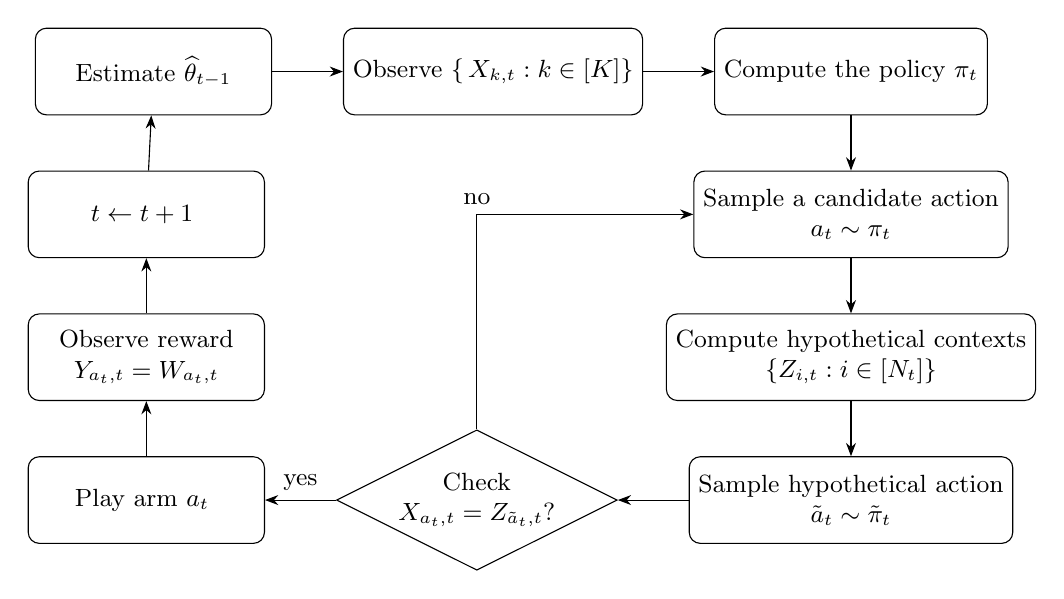
\begin{tikzpicture}[
		>=Stealth,
		node distance = 0.7cm and 0.9cm,
		every node/.style = {font=\small},
		process/.style = {draw, rounded corners, minimum width=30mm, minimum height=11mm, align=center},
		decision/.style = {draw, diamond, aspect=2, inner sep=1pt, align=center}
		]
		
		% Row 1 ---------------------------------------------------------
		\node[process] (theta)   {Estimate $\widehat{\theta}_{t-1}$};
		\node[process, right=of theta]  (observe) {Observe $\{\,X_{k,t}:k\in[K]\}$};
		\node[process, right=of observe]  (pi) {Compute the policy $\pi_t$};
		\node[process, below=of pi] (sampleA) {Sample a candidate action \\ $a_t \sim \pi_t$};
		\node[process, below=of sampleA] (compZ)  {Compute hypothetical contexts \\ $\{Z_{i,t}: i\in[N_t]\}$};
		\node[process, below=of compZ]   (sampleC){Sample hypothetical action \\ $\tilde{a}_t\sim\tilde{\pi}_t$};
		
		% Decision ------------------------------------------------------
		\node[decision, left=of sampleC] (decide)
		{Check \\ $X_{a_t,t}=Z_{\tilde{a}_t,t}$?};
		
		\node[process, left=of decide] (play) 
		{Play arm $a_t$ };
		\node[process, above=of play] (obsr) 
		{ Observe reward \\ $Y_{a_t,t}=W_{a_t,t}$ };
		\node[process, above=of obsr] (inct) 
		{ $t\gets t+1$ };
		% Arrows --------------------------------------------------------
		\draw[->] (theta)   -- (observe);
		\draw[->] (observe) -- (pi);
		\draw[->] (pi) -- (sampleA);
		\draw[->] (sampleA) -- (compZ);
		\draw[->] (compZ)   -- (sampleC);
		\draw[->] (sampleC) -- (decide);
		\draw[->] (decide)  -- node[above]{yes} (play);
		\draw[->] (decide)  |- node[above]{no} (sampleA);  % loop back on "no"
		\draw[->] (play)    -- (obsr);
		\draw[->] (obsr)    -- (inct);
		\draw[->] (inct)    -- (theta);
	\end{tikzpicture}
	\caption{Flow diagram of the proposed coupling and resampling scheme}
	\label{fig:process}
	\vspace{5pt}
\end{figure}

This section introduces a probabilistic method to couple the hypothetical
bandit problem with the original contextual bandit. Figure~\ref{fig:process}
illustrates the overall coupling and resampling process. The key observation
is that the hypothetical pseudo-reward in~\eqref{eq:HDRY} is computable
under the event $\{Z_{\tilde{a}_{s},s}=X_{a_{s},s}\}$, which is implied
by $\{\tilde{a}_{s}=N_{s}\}$. To ensure this condition, we resample
both $a_{s}\sim\pi_{s}$ and $\tilde{a}_{s}\sim\tilde{\pi}_{s}$ using
the distribution in~\eqref{eq:pseudo_prob}.

Each resampling iteration generates updated hypothetical contexts
$\{Z_{i,s}:i\in[N_{s}]\}$, effectively randomizing the hypothetical
contexts and rewards until the pseudo-reward becomes computable. Although
rewards are collected from the original bandit, the estimation of
the parameter $\theta_{\star}$ is performed using compressed and
augmented samples from the hypothetical bandit problem.

Let $\tilde{a}_{s}(m)$ and $a_{s}(m)$ denote the actions sampled
during the $m$-th resampling trial in the hypothetical and original
bandits, respectively. These actions are IID across trials $m$ given
$\Hcal_{t}$. Define the stopping time for successful coupling as
$\xi_{s}:=\inf\{m\geq1:X_{a_{s}(m)}=Z_{\tilde{a}_{s}(m)}\}$. Then,
define the matching event: 
\begin{equation}
\mathcal{M}_{s}:=\{\xi_{s}\leq M_{s}\},\quad M_{s}:=\left\lceil \frac{\log((s+1)^{2}/\delta)}{\log(1/(1-\gamma))}\right\rceil \label{eq:matching_event}
\end{equation}
which ensures a successful coupling within $M_{s}$ trials. Since
$\mathbb{P}(\tilde{a}_{s}(m)=N_{s})=\gamma$, the number of trials
$M_{s}$ is selected to guarantee $\mathbb{P}(\mathcal{M}_{s})\geq1-\delta/(s+1)^{2}$.

The hyperparameter $\gamma$ controls the trade-off: as $\gamma$
increases, the probability of coupling success increases (thus requiring
fewer resampling trials), while the size of the regularization set
$h_{t}$ must increase. Table~\ref{tab:coupling} illustrates the
data structures for successful and failed couplings during resampling.

\begin{table}[t]
\centering %
\begin{tabular}{cccccc}
\toprule 
 & \multicolumn{2}{c|}{Hypothetical Bandit Problem} & \multicolumn{3}{c}{Original Bandit Problem}\tabularnewline
\midrule 
 & Arm 1  & Arm 2  & Arm 1  & Arm 2  & Arm 3 \tabularnewline
\midrule 
Failure  & \cellcolor{Gray}$(Z_{\tilde{a}_{t},t},W_{\tilde{a}_{t},t})$  & $(Z_{N_{t},t},?)$  & $(X_{1,t},?)$  & $(X_{2,t},?)$  & \cellcolor{Gray}$(X_{a_{t},t},Y_{a_{t},t})$ \tabularnewline
\midrule 
Success  & $(Z_{1,t},?)$  & \cellcolor{Gray}$(Z_{N_{t},t},W_{N_{t},t})$  & $(X_{1,t},?)$  & \cellcolor{Gray}$(X_{a_{t},t},Y_{a_{t},t})$  & $(X_{3,t},?)$ \tabularnewline
\bottomrule
\end{tabular}\caption{Illustration of coupling success and failure during resampling for
$N_{t}=2$ and $K=3$. By construction, $Z_{2,t}:=X_{a_{t},t}$ and
$W_{2,t}:=Y_{a_{t},t}$. Gray cells indicate the selected actions.}
\label{tab:coupling} 
\end{table}

%------------------ Sub-algorithm ------------------
\begin{algorithm}[t]
\caption{Candidate-Arm Sampler (\texttt{CAS}) for Round $t$}
\label{alg:cas} \begin{algorithmic}[1] \STATE \textbf{Input:}
contexts $\{X_{k,t}\}_{k\in[K]}$, posterior mean $\widehat{\theta}_{t-1}$,
exploration variance $v_{t-1}$, Gram matrix $V_{t-1}$, pseudo-index
$N_{t}$, coupling parameter $\gamma$, confidence $\delta$. \STATE
\textbf{Set} $M_{t}$ as in~\eqref{eq:matching_event} \hfill{}\COMMENT{//
maximum retries} \STATE \textbf{Initialise} $m\gets1$ \REPEAT
\STATE Sample $\tilde{\theta}_{k,t}^{(m)}\sim\mathcal{N}\!\bigl(\widehat{\theta}_{t-1},\,v_{t-1}^{2}V_{t-1}^{-1}\bigr)$
independently for all $k\in[K]$ \STATE $a_{t}^{(m)}\gets\arg\max_{k\in[K]}X_{k,t}^{\top}\tilde{\theta}_{k,t}^{(m)}$
\STATE Sample $\tilde{a}_{t}^{(m)}$ from the distribution in~\eqref{eq:pseudo_prob}
\STATE $m\gets m+1$ \UNTIL{$\tilde{a}_{t}^{(m-1)}=N_{t}\;\;\mathbf{or}\;\;m>M_{t}$}
\STATE \textbf{Output:} $a_{t}^{\star}\gets a_{t}^{(m-1)}$, \quad{}$\tilde{a}_{t}^{\star}\gets\tilde{a}_{t}^{(m-1)}$
\end{algorithmic} 
\end{algorithm}

%----------------------------------------------------

The proposed resampling-coupling scheme is describe in Algorithm~\ref{alg:cas}
as candidate arm sampler (\texttt{CAS}). The resampling in \texttt{CAS}
is distinctive from that in \citet{kim2021doubly} and \citet{xu2020upper}.
The resampling in \citet{kim2021doubly} resamples the action to find
the arm whose selection probability is greater than a prespecified
threshold value. \citet{xu2020upper} resamples the previous counterfactual
actions and contexts to impose randomization and generalization on
the estimator. In contrast, our resampling is to couple the hypothetical
samples with the original samples and this coupling is the first method
a novel innovative part in this work.

Upon obtaining the coupled contexts $Z_{\tilde{a}_{s}(M_{s}),s}=X_{a_{s}(M_{s}),s}$,
we construct the coupled pseudo-reward as: 
\begin{equation}
W_{i,s}^{Co(\check{\theta}_{t})}:=\left(1-\frac{\mathbb{I}(\tilde{a}_{s}(M_{s})=i)}{\phi_{i,s}}\right)Z_{i,s}^{\top}\check{\theta}_{t}+\frac{\mathbb{I}(\tilde{a}_{s}(M_{s})=i)}{\phi_{i,s}}W_{i,s},\label{eq:CoY}
\end{equation}
which is computable for all $i\in[N_{s}]$ because $a_{s}(M_{s})$
is selected and $W_{\tilde{a}_{s}(M_{s}),s}=Y_{a_{s}(M_{s}),s}$ is
observable.

Given an reference estimator $\check{\theta}_{t}$ defined in~\eqref{eq:impute},
the proposed \emph{hypothetical coupled sample augmented} (HCSA) estimator
is defined as: 
\begin{equation}
\widehat{\theta}_{t}:=\left\{ \sum_{s=1}^{t}\mathbb{I}(\mathcal{M}_{s})\sum_{i=1}^{N_{s}}Z_{i,s}Z_{i,s}^{\top}\right\} ^{-1}\left(\sum_{s=1}^{t}\mathbb{I}(\mathcal{M}_{s})\sum_{i=1}^{N_{s}}W_{i,s}^{Co(\check{\theta}_{t})}Z_{i,s}\right).\label{eq:A_estimator}
\end{equation}
The indicator $\II(\Mcal_{s})$ makes the estimator use the coupled
pseudo-rewards~\eqref{eq:CoY} only when $\mathcal{M}_{s}$ occurs;
otherwise, it skips round $s$ and relies on the previous estimator.
Since $\mathcal{M}_{s}$ occurs with high probability, we can couple
the HCSA estimator with the hypothetical sample augmented estimator
from~\eqref{eq:Hypo_DR}.

While the DR estimator in~\eqref{eq:DR_estimator} where the $K$
pseudo-rewards are augmented, the proposed (HCSA) estimator~\eqref{eq:Hypo_DR}
adds $N_{s}\le d+1$ for each round $s\in[t]$. This reduction in
the number of augmented pseudo-reward samples paves a way to reduce
the error and eliminate the IID and minimum eigenvalue assumption
on contexts, by which \citet{kim2021doubly} used to obtain a regret
bound that depends on the minimum eigenvalue of the context covariance.

Next, we provide a coupling inequality that relates the HCSA estimator
to hypothetical sample augmented estimator $\tilde{\theta}_{t}^{H(\check{\theta}_{t})}$.
\begin{lemma}[A coupling inequality] \label{lem:coupling} For
$t\geq1$, let $\Scal_{t}:=\cap_{s=1}^{t}\Mcal_{s}$, where $\Mcal_{s}$
is the matching event defined in~\eqref{eq:matching_event}. For
the reference estimator $\check{\theta}_{t}$ defined in~\eqref{eq:impute}
and for $x>0$, 
\[
\PP\left(\left\{ \norm{\widehat{\theta}_{t}^{A(\check{\theta}_{t})}-\theta_{\star}}_{\Gb_{t}}>x\right\} \right)\leq\PP\left(\left\{ \norm{\tilde{\theta}_{t}^{H(\check{\theta}_{t})}-\theta_{\star}}_{\Gb_{t}}>x\right\} \cap\Scal_{t}\right)+\PP(\Scal_{t}^{c}),
\]
and the failure probability satisfies $\PP(\Scal_{t}^{c})\leq\delta$.
\end{lemma}
\begin{proof}
Fix $t\in[T]$ throughout the proof. For any $\check{\theta}\in\RR^{d}$
and $x>0$, decompose the probability as follows: 
\[
\PP\left(\norm{\widehat{\theta}_{t}-\theta_{\star}}_{\Gb_{t}}>x\right)\leq\PP\left(\left\{ \norm{\widehat{\theta}_{t}-\theta_{\star}}_{\Gb_{t}}>x\right\} \cap\Scal_{t}\right)+\PP\left(\Scal_{t}^{c}\right).
\]
On the event $\Scal_{t}:=\cap_{s=1}^{t}\Mcal_{s}$, the HCSA estimator
in~\eqref{eq:A_estimator} is simplified to 
\[
\widehat{\theta}_{t}^{A(\check{\theta}_{t})}=\left\{ \sum_{s=1}^{t}\sum_{i=1}^{N_{s}}Z_{i,s}Z_{i,s}^{\top}\right\} ^{-1}\left(\sum_{s=1}^{t}\sum_{i=1}^{N_{s}}W_{i,s}^{Co(\check{\theta}_{t})}Z_{i,s}\right)=\Gb_{t}\left(\sum_{s=1}^{t}\sum_{i=1}^{N_{s}}W_{i,s}^{Co(\check{\theta}_{t})}Z_{i,s}\right).
\]
Define the function 
\[
F\Bigl(\tilde{a}_{1}(M_{1}),\ldots,\tilde{a}_{t}(M_{t})\Bigr):=\norm{\widehat{\theta}_{t}-\theta_{\star}}_{\Gb_{t}}=\norm{\sum_{s=1}^{t}\sum_{i=1}^{N_{s}}(W_{i,s}^{Co(\check{\theta}_{t})}-Z_{i,s}^{\top}\theta_{\star})Z_{i,s}}_{\Gb_{t}}.
\]
Using the definition of $M_{s}$, where $\tilde{a}_{s}(M_{s})=N_{s}$,
we have 
\begin{align*}
 & \PP\left(\left\{ F\Bigl(\tilde{a}_{1}(M_{1}),\ldots,\tilde{a}_{t}(M_{t})\Bigr)>x\right\} \cap\Scal_{t}\right)\\
 & =\PP\left(\left\{ F\Bigl(\tilde{a}_{1}(M_{1}),\ldots,\tilde{a}_{t}(M_{t})\Bigr)>x\right\} \cap\Scal_{t}\cap\bigcap_{s=1}^{t}\{\tilde{a}_{s}(M_{s})=N_{s}\}\right)\\
 & =\PP\left(\left\{ F\Bigl(\tilde{a}_{1}(1),\ldots,\tilde{a}_{t}(1)\Bigr)>x\right\} \cap\Scal_{t}\cap\bigcap_{s=1}^{t}\{\tilde{a}_{s}(1)=N_{s}\}\right),
\end{align*}
where the last equality holds because $\{\tilde{a}_{s}(m):m\in\NN\}$
are IID for each $s\in[t]$. Then, 
\begin{align*}
 & \PP\left(\left\{ F\Bigl(\tilde{a}_{1}(1),\ldots,\tilde{a}_{t}(1)\Bigr)>x\right\} \cap\Scal_{t}\cap\bigcap_{s=1}^{t}\{\tilde{a}_{s}(1)=N_{s}\}\right)\\
 & \leq\PP\left(\left\{ F\Bigl(\tilde{a}_{1}(1),\ldots,\tilde{a}_{t}(1)\Bigr)>x\right\} \cap\Scal_{t}\right)
\end{align*}
Replacing $\{\tilde{a}_{s}(M_{s}):s\in[t]\}$ in coupled pseudo-rewards~\eqref{eq:CoY}
with $\{\tilde{a}_{s}(1):s\in[t]\}$ gives the hypothetical pseudo-rewards
in~\eqref{eq:HDRY}. Thus, the distribution of the normalized error
$\|\tilde{\theta}_{t}^{H(\check{\theta}_{t})}-\theta_{\star}\|_{\Gb_{t}}$
is equivalent to that of $F\bigl(\tilde{a}_{1}(1),\ldots,\tilde{a}_{t}(1)\bigr)$
and we obtain 
\[
\PP\Big(\big\{ F\bigl(\tilde{a}_{1}(1),\ldots,\tilde{a}_{t}(1)\bigr)>x\big\}\cap\Scal_{t}\Big)=\PP\Big(\big\{\|\tilde{\theta}_{t}^{H(\check{\theta}_{t})}-\theta_{\star}\|_{\Gb_{t}}>x\big\}\cap\Scal_{t}\Big),
\]
which proves the coupling inequality. The bound for the failure probability
$\PP(\Scal_{t}^{c})\le\delta$ is proved by the fact that $\PP(\Mcal_{s}^{c})\le\delta/(s+1)^{2}$
by construction of the maximum number of resampling trials. 
\end{proof}
With the coupling inequality, we can leverage augmented samples from
the hypothetical bandit problem to closely approximate the hypothetical
sample augmented estimator with high probability. While the coupling
technique can be applied to any choice of hypothetical problem ---
and the hypothetical contexts $\{Z_{i,t}\}$ may be arbitrarily defined
--- it is crucial that they are compatible with the original contextual
bandit problem and the reference estimator $\check{\theta}_{t}$.

The design of suitable hypothetical contexts is key, as it enables
control of the maximum deviation in the original problem through the
bound: 
\[
\max_{k\in[K]}\left|X_{k,t}^{\top}\left(\tilde{\theta}_{t}^{H(\check{\theta}_{t})}-\theta_{\star}\right)\right|\le\norm{\tilde{\theta}_{t}^{H(\check{\theta}_{t})}-\theta_{\star}}_{\tilde{G}_{t}}\cdot\max_{k\in[K]}\norm{X_{k,t}}_{\tilde{G}_{t}^{-1}},
\]
where $\tilde{G}_{t}:=\sum_{s=1}^{t}\sum_{i=1}^{N_{s}}Z_{i,s}Z_{i,s}^{\top}$
denotes the Gram matrix constructed from the hypothetical contexts.

This upper bound consists of two components: (i) the self-normalized
error of the hypothetical sample augmented estimator, and (ii) the
maximum norm of the original contexts normalized by $\tilde{G}_{t}$.
Each component is sensitive to how the Gram matrix $\tilde{G}_{t}$
is constructed.

If $\tilde{G}_{t}$ is defined using only the played contexts ---
i.e., $\tilde{G}_{t}=\sum_{s=1}^{t}X_{a_{s},s}X_{a_{s},s}^{\top}+I_{d}$
--- then the norm term $\max_{k\in[K]}\|X_{k,t}\|_{\tilde{G}_{t}^{-1}}$
may become unbounded due to insufficient exploration. Conversely,
if $\tilde{G}_{t}$ is constructed from an overly large set of hypothetical
contexts, the self-normalized error $\|\tilde{\theta}_{t}^{H(\check{\theta}_{t})}-\theta_{\star}\|_{\tilde{G}_{t}}$
may increase significantly, making it harder to guarantee tight estimation
bounds.

Therefore, the design of the hypothetical contexts must carefully
balance the number of augmenting samples to ensure both the estimator's
accuracy and the tightness of high-probability bounds. Section~\ref{sec:self}
presents a formal analysis of this trade-off, and shows that the proposed
construction achieves this balance effectively, leading to a well-conditioned
estimator with high-probability regret guarantees.

\subsection{Hypothetical Coupled Sample Augmented Thompson Sampling}

\label{sec:algorithm}

\begin{algorithm}[t]
\caption{Hypothetical Coupled Sample Augmented Thompson Sampling (\texttt{HCSA+TS})}
\label{alg:ATS} \begin{algorithmic}[1] \STATE \textbf{Input:}
confidence level $\delta\in(0,1)$, coupling parameter $\gamma\in(0,1)$,
exploration parameter $\Gb_{t}:=\{2\log\frac{K(t+1)^{2}}{\delta}\}^{-1/2}$,
orthogonal basis regularization parameter $h_{t}$ as in~\eqref{eq:h_t}.
\STATE Initialize the estimator $\widehat{\theta}_{0}=\mathbf{0}$,
Gram matrix $V_{0}=O$, and a subset of rounds for the orthogonal
basis regularization $\mA_{0}=\emptyset$. \FOR{$t=1$ \textbf{to}
$T$} \STATE Observe contexts $\{X_{k,t}:k\in[K]\}$. \STATE Update
$\Acal_{t}$ as in \eqref{eq:A} and compute $N_{t}$ as in \eqref{eq:N}.
\STATE Set $m=1$ sample $\tilde{a}_{t}(m)$ from the multinomial
distribution \eqref{eq:pseudo_prob}. \STATE $(a_{t}(m),\tilde{a}_{t}(m))\gets\texttt{CAS}\bigl(\{X_{k,t}\},\widehat{\theta}_{t-1},v_{t-1},V_{t-1},N_{t},\gamma,\delta\bigr)$
\IF{$\tilde{a}_{t}(m)=N_{t}$ // Resampling succeeded} \STATE
Pull arm $a_{t}(m)$ and observe $Y_{a_{t}(m),t}$. \STATE Compute
the reference estimator $\check{\theta}_{t}$ defined in~\eqref{eq:impute}.
\IF{$t\in\Acal_{t}$} \STATE Compute hypothetical contexts $Z_{i,t}:=H_{i,t}$
as in \eqref{eq:new_contexts} \ELSE \STATE Compute hypothetical
contexts $Z_{i,t}:=\tilde{H}_{i,t}$ with orthogonal basis as in \eqref{eq:new_contexts}.
\ENDIF \STATE Update $\Gb_{t}=V_{t-1}+\sum_{i=1}^{N_{t}}Z_{i,s}Z_{i,s}^{\top}$
\STATE Compute the estimator $\widehat{\theta}_{t}$ as in ~\eqref{eq:A_estimator}.
\ELSE \STATE $\widehat{\theta}_{t}\leftarrow\widehat{\theta}_{t-1}$
\ENDIF \ENDFOR \end{algorithmic} 
\end{algorithm}

The proposed algorithm, \textit{Hypothetical Coupled Sample Augmented
Thompson Sampling} (\texttt{HCSA+TS}), is detailed in Algorithm \ref{alg:ATS}.
This algorithm builds upon the structure of \texttt{LinTS} but introduces
two key innovations: (i) resampling to couple the hypothetical bandit
with the original bandit, and (ii) the HCSA estimator, which leverages
a compressed orthogonal basis for improved efficiency.

For the resampling step (i), the algorithm repeatedly resamples $a_{t}$
from \texttt{LinTS} policy equipped with HCSA estimator and the novel
Gram matrix until the condition $\{Z_{\tilde{a}_{t},t}=X_{a_{t},t}\}$
is satisfied. This ensures that the hypothetical bandit aligns with
the original bandit by augmenting the randomized contexts. The number
of resampling attempts, set to $\lceil\log\frac{(t+1)^{2}}{\delta}/\log\frac{1}{1-\gamma}\rceil$,
guarantees the resampling process succeeds with probability at least
$1-\delta/(t+1)^{2}$. In practice, this resampling typically succeeds
after only a few iterations.

For the HCSA estimator (ii), although computing it might appear computationally
demanding, efficient implementation strategies significantly reduce
its complexity. Theoretically, the algorithm must compute hypothetical
context vectors $\{Z_{i,t}:i\in[N_{t}]\}$ for each resampling iteration.
However, in practice, the algorithm first checks if $\{\tilde{a}_{t}=N_{t}\}$
occurs and then computes the hypothetical contexts based on the resampled
$a_{t}$.

The worst-case computational complexity of the algorithm is $O(d^{2}(K+d)T+T\log(T+1)/\log(\frac{1}{1-\gamma}))$.
The primary computational bottleneck arises from calculating the Gram
matrix $\Gb_{t}$ and performing eigenvalue decomposition to construct
hypothetical contexts, repeated for the specified number of resampling
attempts in each round $t\in[T]$. In practice, the computational
efficiency of the A estimator can be further enhanced by applying
the Sherman-Morrison formula, enabling rank-1 updates and reducing
memory usage.

%-------------------------------------------
% 5. Regret Analysis
%-------------------------------------------

\section{Regret Analysis}

\label{sec:regret_analysis} The following theorem establishes a nearly
minimax-optimal cumulative regret bound for the \texttt{HCSA+TS} algorithm.

\begin{theorem}[Regret Bound for \texttt{HCSA+TS}] 
	\label{thm:regret_bound}
In Algorithm~\ref{alg:ATS}, set the exploration parameter as $\Gb_{t}=\{2\log(K(t+1)^{2}/\delta)\}^{-1/2}$.
Then, with probability at least $1-3\delta$, the cumulative regret
of the \texttt{HCSA+TS} algorithm by round $T$ satisfies: 
\begin{equation}
R(T)\leq\frac{4d}{(1/2-e^{-1})(1-\gamma)}\log\frac{d(T+1)^{2}}{\delta}+\left\{ 20\sqrt{2}\theta_{\max}+\frac{21\sigma}{\gamma}\sqrt{2d\log\frac{2T}{\delta}}+1\right\} \sqrt{8dT\log\frac{T}{d}}.\label{eq:regret_bound}
\end{equation}
\end{theorem}

The leading order term of the regret bound is $O(d\sqrt{T}\log T)$,
which matches the minimax lower bound $\Omega(d\sqrt{T})$ established
in \citet{lattimore2020bandit}, up to logarithmic factors. This result
provides the first nearly minimax-optimal regret guarantee for linear
contextual bandits under arbitrary context distributions.

For comparison, \cite{kim2021doubly} achieved $\tilde{O}(d\sqrt{T})$
regret bound under IID contexts with some special distributions of
which the minimum eigenvalue of the average covariance matrix is $\Omega(1/d)$.
\citet{kim2023squeeze} achieved a regret bound of $O(\sqrt{dT\log T})$
under the assumption of IID contexts with a strictly positive minimum
eigenvalue for their average covariance matrix. Similarly, \citet{huix2023tight}
obtained a regret bound of $\tilde{O}(d\sqrt{T})$, but their analysis
assumes a Gaussian prior on the unknown parameter $\theta_{\star}$.

Earlier works such as \citet{kim2021doubly} and \citet{agrawal2013thompson}
impose unit-norm assumptions on the contexts. In contrast, the regret
bound~\eqref{eq:regret_bound} does not require normalization of
the context vectors. The only assumption made is that the absolute
inner product between any context and the true parameter is bounded,
i.e., $|X_{k,t}^{\top}\theta_{\star}|\leq1$. Notably, increasing
the context norm bound $x_{\max}$ does not cause the regret to grow
linearly, avoiding the scaling issues encountered in prior analyses.

The key technical contributions enabling this result include: (i)
the development of a self-normalized bound for the HCSA estimator
using a carefully constructed Gram matrix (Section~\ref{sec:self}),
(ii) the identification of a set of low-regret arms selected with
high probability (Section~\ref{sec:low_regret_arms}), and (iii)
a novel maximal elliptical potential bound based on the augmented
Gram matrix $\Gb_{t}$ (Section~\ref{sec:max_elliptical}).

\subsection{A Self-Normalized Bound for the Proposed Estimator}

\label{sec:self} With the coupling inequality (Lemma~\ref{lem:coupling}),
we can bound the error of the proposed estimator by obtaining an error
bound for the hypothetical estimator~\eqref{eq:Hypo_DR}, which is
proven in the following lemma.

\begin{lemma}[A self-normalized bound of the HSA estimator] \label{lem:error_decomposition}
For each $t\ge1$, define the matrix $A_{t}:=\sum_{s=1}^{t}\phi_{\tilde{a}_{s},s}^{-1}Z_{\tilde{a}_{s},s}Z_{\tilde{a}_{s},s}^{\top}$.
and. Then the self-normalized bound of the hypothetical sample augmented
estimator is decomposed as: 
\[
\norm{\tilde{\theta}_{t}^{H(\check{\theta}_{t})}-\theta_{\star}}_{\Gb_{t}}\le\norm{\Gb_{t}^{-1/2}(\Gb_{t}-A_{t})(\check{\theta}_{t}-\theta_{\star})}_{2}+\norm{\sum_{s=1}^{t}\phi_{\tilde{a}_{s},s}^{-1}(W_{\tilde{a}_{s},s}-Z_{\tilde{a}_{s},s}^{\top}\theta_{\star})Z_{\tilde{a}_{s},s}}_{\Gb_{t}}
\]
\end{lemma}

The proof is in Appendix~\ref{sec:error_decomposition_proof}. The
decomposition shows the two sources of error for the HDR estimator
for rewards of all arms: (i) from the reference estimator $\check{\theta}$
used as an reference estimator in HDR pseudo-rewards~\eqref{eq:HDRY},
and (ii) the noise error of the rewards. In error term (i), $\Gb_{t}(\Gb_{t}-A_{t})$
is the matrix martingale with bounded eigenvalues, which is bounded
by the newly developed matrix concentration inequality (Lemma \ref{lem:matrix_neg}).
The error term (ii) is bounded by a modified martingale inequality
developed by \citet{abbasi2011improved}.

With the suitable choice of $\check{\theta}_{t}$ as in~\eqref{eq:impute},
we obtain an $O(\sqrt{d\log t})$ error bound for $\tilde{\theta}_{t}^{H(\check{\theta}_{t})}$
estimator, which is normalized by the novel augmented Gram matrix
$\Gb_{t}$ instead of the conventional Gram matrix that includes only
selected contexts.

\begin{theorem}[A Self-Normalized Bound for the HCSA Estimator] The
HCSA estimator~\eqref{eq:A_estimator} satisfies, 
\[
\norm{\widehat{\theta}_{t}-\theta_{\star}}_{\Gb_{t}}\leq20\theta_{\max}+\frac{21\sigma}{\gamma}\sqrt{d\log\frac{1+t}{\delta}},
\]
with probability at least $1-3\delta$ for all $t\geq T_{1}$. \label{thm:self}
\end{theorem} The proof is provided in Appendix~\ref{sec:tail_proof}.
Unlike the conventional self-normalized bound of \citet{abbasi2011improved},
which is normalized by the Gram matrix $\sum_{s=1}^{t}X_{a_{s},s}X_{a_{s},s}^{\top}+I_{d}$
built solely from selected contexts, Theorem~\ref{thm:self} establishes
a bound normalized by the full Gram matrix $\Gb_{t}$, which includes
contexts from all $K$ arms. While \citet{kim2023squeeze} also considered
self-normalization with respect to a full Gram matrix, their estimator
incorporates contexts from all arms only in a fraction of the rounds,
and their analysis is restricted to IID contexts with a strictly positive-definite
covariance matrix. In contrast, Theorem~\ref{thm:self} applies to
arbitrary (including non-IID, non-stationary) context sequences, establishing
a uniform self-normalized bound with a full Gram matrix. This result
enables a novel regret analysis of Thompson Sampling that yields a
$\tilde{O}(d\sqrt{T})$ bound for \texttt{HCSA+TS}, applicable under
arbitral context distributions.

\subsection{Low-Regret Arms with a High-Probability Guarantee}

\label{sec:low_regret_arms} For each $k\in[K]$ and $t\in[T]$, define
the instantaneous regret gap between the optimal arm and arm $k$
as 
\[
\Delta_{k,t}:=X_{a_{t}^{\star},t}^{\top}\theta_{\star}-X_{k,t}^{\top}\theta_{\star}.
\]
Using this, we define the set of low-regret arms at round $t$ as
\begin{equation}
\mathcal{P}_{t}:=\left\{ k\in[K]:\Delta_{k,t}\le2x_{t}\norm{\widehat{\theta}_{t-1}-\theta_{\star}}_{\Gb_{t-1}}+\sqrt{\norm{X_{a_{t}^{\star},t}}_{\Gb_{t-1}^{-1}}^{2}+\norm{X_{k,t}}_{\Gb_{t-1}^{-1}}^{2}}\right\} ,\label{eq:low_regret_set}
\end{equation}
where $x_{t}:=\max_{k\in[K]}\|X_{k,t}\|_{\Gb_{t-1}^{-1}}$. The self-normalized
confidence bound with respect to the hypothetical Gram matrix $\Gb_{t-1}$,
which includes contexts beyond the selected arms, allows the construction
of an effective set $\mathcal{P}_{t}$ that has lower regret than
arms in sets built from Gram matrices based solely on selected contexts
such as $\sum_{s=1}^{t}X_{a_{s},s}X_{a_{s},s}^{\top}+I_{d}$.

The following lemma provides a high-probability guarantee that the
arm selected by Algorithm~\ref{alg:ATS} belongs to the low-regret
set. \begin{lemma}[High-Probability Selection of Low-Regret Arms]
\label{lem:super_unsaturated_arms} Let $a_{t}$ be the arm selected
by Algorithm~\ref{alg:ATS}, and let $\mathcal{P}_{t}$ be the set
defined in~\eqref{eq:low_regret_set}. If the exploration parameter
is set as $\Gb_{t}=\{2\log(K(t+1)^{2}/\delta)\}^{-1/2}$, then 
\[
\mathbb{P}\left(a_{t}\in\mathcal{P}_{t}\mid\mathcal{H}_{t}\right)\ge1-\frac{\delta}{(t+1)^{2}}.
\]
\end{lemma} The proof is deferred to Appendix~\ref{sec:low_regret_proof}.
In contrast to \citet{agrawal2013thompson}, where bounding the probability
of selecting a saturated arm required setting $v=\sqrt{9d\log(t/\delta)}$,
thereby introducing a $\sqrt{d}$-scaling, Lemma~\ref{lem:super_unsaturated_arms}
establishes that such dimensional dependence is unnecessary. By leveraging
the structure of the HCSA estimator and its associated Gram matrix,
the proposed approach guarantees high-probability selection of low-regret
arms without incurring additional dependence of the variance parameter
$v$ on the dimension $d$

\subsection{Maximal Elliptical Potential Bound}

\label{sec:max_elliptical} While continuing the proof of the regret
bound, we face a novel terms that needs to be analyzed. By Lemma~\ref{lem:super_unsaturated_arms},
the algorithm selects arms from the low-regret set $\Pcal_{t}$, i.e.,
$a_{t}\in\Pcal_{t}$, with high probability. This leads to the following
novel regret decomposition:

\[
\Regret{t}=\Diff{a_{t}}{t}\leq2x_{t}\norm{\Estimator{t-1}-\theta_{\star}}_{\Gb_{t-1}}+\sqrt{\norm{X_{a_{t}^{\star},t}}_{\Gb_{t-1}^{-1}}^{2}+\norm{X_{a_{t},t}}_{\Gb_{t-1}^{-1}}^{2}},
\]
for $t\geq T_{1}$. Thus, the cumulative regret is bounded as follows:
\[
R(T)\leq2h_{T}+\sum_{t\in[T]\setminus\Acal_{T}}\left\{ 2x_{t}\norm{\Estimator{t-1}-\theta_{\star}}_{\Gb_{t-1}}+\sqrt{\norm{X_{a_{t}^{\star},t}}_{\Gb_{t-1}^{-1}}^{2}+\norm{X_{a_{t},t}}_{\Gb_{t-1}^{-1}}^{2}}\right\} .
\]
Because $x_{t}:=\max_{k\in[K]}\|X_{k,t}\|_{V_{t-1}^{-1}}$, we get:
\[
R(T)\leq2h_{T}+\sum_{t\in[T]\setminus\Acal_{T}}\big(2x_{t}\|\Estimator{t-1}-\theta_{\star}\|_{\Gb_{t-1}}+\sqrt{2}x_{t}\big).
\]
Factoring out $x_{t}$: 
\[
R(T)\leq2T_{1}+\sum_{t=\in[T]\setminus\Acal_{T}}\big(2\|\Estimator{t-1}-\theta_{\star}\|_{\Gb_{t-1}}+\sqrt{2}\big)x_{t}.
\]
Since we obtain $\|\Estimator{t-1}-\theta_{\star}\|_{V_{t-1}}=O(\sqrt{d\log t})$
from Theorem~\ref{thm:self}, we need a bound for $\sum_{t\in[T]\setminus\Acal_{T}}x_{t}$,
which is in the following lemma.

\begin{lemma}[Maximal elliptical potential lemma] \label{lem:elliptical}
For $x_{t}:=\max_{k\in[K]}\|X_{k,t}\|_{\Gb_{t-1}^{-1}}$, we have:
\[
\sum_{t=T_{1}}^{T}x_{t}^{2}\leq4d\log\frac{T}{d}.
\]
\end{lemma} The proof is in Appendix~\ref{sec:proof_elliptical}.
Previous elliptical lemmas only obtain the bounds the normalized norm
of the selected contexts $X_{a_{t},t}$, while we need a bound for
$\max_{k\in{K]}}\|X_{k,t}\|_{\Gb_{t-1}^{-1}}$. The maximal elliptical
potential lemma bounds the normalized norm of the contexts for all
$K$ arms, which previous analyses could not bound effectively. This
is possible because we augmented suitable sample to obtain the Gram
matrix $\Gb_{t}$ consisting of contexts from all $K$ arms.

%-------------------------------------------
% 6. Experimental Results
%-------------------------------------------


\section{Experimental Results}

\label{sec:experiment} This section is for evaluating the empirical
performance of the proposed algorithm, \texttt{HCSA+TS}, against several
benchmark algorithms for LinCB with simulated data. The benchmarks
include \texttt{LinTS}, \texttt{LinUCB}, \texttt{DRTS} \citep{kim2021doubly},
\texttt{HyRan} \citep{kim2023squeeze}, and \texttt{SupLinUCB} \citep{chu2011contextual}.

%----------------------------------------
% Figure 1. Regret comparison
%----------------------------------------
\begin{figure}[t]
\centering \subfigure[Regret comparison ($d=10$, $K=20$)]{{\includegraphics[width=0.48\textwidth]{figures/Regrets_10dimension_20arms}
}} \subfigure[Regret comparison ($d=30$, $K=20$)]{{\includegraphics[width=0.48\textwidth]{figures/Regrets_30dimension_20arms}
}} \\
 \subfigure[Regret comparison ($d=10$, $K=30$)]{{\includegraphics[width=0.48\textwidth]{figures/Regrets_10dimension_30arms}
}} \subfigure[Regret comparison ($d=30$, $K=30$)]{{\includegraphics[width=0.48\textwidth]{figures/Regrets_30dimension_30arms}
}} \caption{ Comparison of the regrets of the proposed \texttt{HCSA+TS} algorithm
with other benchmark methods. The lines represent the average, and
the shaded areas indicate the standard deviation based on twenty experiments.
The results demonstrate that the proposed \texttt{HCSA+TS} effectively
identifies the optimal arm using orthogonal regularization.}\label{fig:comparison}
\end{figure}

%----------------------------------------
% Figure 2. Prediction error
%----------------------------------------
\begin{figure}[t]
\centering \subfigure[Prediction error comparison ($d=10$, $K=20$)]{{\includegraphics[width=0.48\textwidth]{figures/est_10dimension_20arms}
}} \hfill{}\subfigure[Prediction error comparison ($d=30$, $K=20$)]{{\includegraphics[width=0.48\textwidth]{figures/est_30dimension_20arms}
}} \\
 \subfigure[Prediction error comparison ($d=10$, $K=30$)]{{\includegraphics[width=0.48\textwidth]{figures/est_10dimension_30arms}
}} \hfill{}\subfigure[Prediction error comparison ($d=30$, $K=30$)]{{\includegraphics[width=0.48\textwidth]{figures/est_30dimension_30arms}
}} %\vspace{.1in}
\caption{ Comparison of the prediction error across all arms, calculated as
$\sum_{i=1}^{K}\{X_{i,t}^{\top}(\widehat{\theta}_{t}-\theta_{\star})\}^{2}$,
for the proposed \texttt{HCSA+TS} and other benchmark methods. The
lines represent the averages, and the shaded areas indicate the standard
deviations based on twenty experiments. The results demonstrate that
the proposed estimator, enhanced with orthogonal augmentation, learns
the reward more accurately than other estimators.}\label{fig:prediction}
\end{figure}

For the experiment setting, the parameter $\theta_{\star}$ is defined
as: 
\[
\theta_{\star}:=\frac{1}{\sqrt{d}}\biggl(\underset{\lceil d/2\rceil}{\underbrace{1,\cdots,1}},\underset{d-\lceil d/2\rceil}{\underbrace{-1,\cdots,-1}}\biggr)^{\top},
\]
where $d\in\{10,30\}$ is the dimension of the parameter. The $i$-th
entry of the context vectors for $K\in\{20,30\}$ arms are independently
sampled from a Gaussian distribution with a mean of $-1+\frac{3(i-1)}{d-1}$
and variance of 1 for each $i\in[d]$. These vectors are normalized
and then scaled by a scalar drawn uniformly from $[0,1]$. To simulate
missing context information, with probability $1/2$, the last $d-\lceil d/2\rceil$
entries of the context vectors are set to zero at each round. This
setting reflects practical scenarios where certain context features
may be unavailable with some probability, making it challenging to
estimate the corresponding entries in $\theta_{\star}$.

The hyperparameter optimization was conducted as follows: For \texttt{LinTS},
the variance parameter was selected from $\{0.01,0.1,1\}$. For \texttt{LinUCB}
and \texttt{SupLinUCB}, the confidence bound inflation parameter was
chosen from $\{0.01,0.1,1\}$. For \texttt{HyRan} and \texttt{HCSA+TS},
the regularization parameters $p$ and $\gamma$ (only $\gamma$ for
\texttt{HCSA+TS}) were tuned from $\{0.1,0.5,0.9\}$. The hyperparameters
for \texttt{DRTS} were fixed as specified in \citet{kim2021doubly}.
Values outside the specified ranges showed negligible differences
in performance, suggesting robustness to hyperparameter selection
for all methods.

Figure~\ref{fig:comparison} compares the cumulative regret of \texttt{HCSA+TS}
with other benchmark algorithms across various configurations of $d$
and the number of arms $K$. Each line represents the average cumulative
regret, and the shaded regions indicate the standard deviation across
20 independent trials.

The results show that \texttt{HCSA+TS} achieves the lowest cumulative
regret in all tested settings. Compared to \texttt{LinTS}, \texttt{LinUCB},
and \texttt{SupLinUCB}, which do not leverage information from all
arms, \texttt{HCSA+TS} demonstrates robustness to missing context
data. When compared to \texttt{DRTS} and \texttt{HyRan}, which uses
the original context vectors, \texttt{HCSA+TS} consistently identifies
low-regret arms more effectively, even under significant masking of
context features.

Initially, due to the orthogonal basis regularization, \texttt{HCSA+TS}
incurs higher regret during the exploration phase, particularly when
the effective rank of the context matrix is low. However, it rapidly
adapts and identifies the optimal arm, ultimately outperforming the
other algorithms, which continue to suffer regret due to their inability
to handle missing context data effectively.

Figure~\ref{fig:prediction} illustrates the prediction error across
all arms, measured as $\sum_{i=1}^{K}\{X_{i,t}^{\top}(\widehat{\theta}_{t}-\theta_{\star})\}^{2}$.
Similar to the regret results, the averages and standard deviations
are computed over 20 trials. The initial convergence of the estimators
in \texttt{DRTS} and \texttt{HyRan} is faster due to their reliance
on imputed contexts. However, their prediction errors increase over
time because the imputed contexts, often containing many zero entries,
provide incomplete information and hinder accurate estimation. In
contrast, \texttt{HCSA+TS} demonstrates steady and consistent convergence
throughout the experimental horizon. Its orthogonal augmentation strategy
allows it to extract useful information even when parts of the context
vectors are masked, leading to superior prediction accuracy compared
to both traditional ridge-based estimators (\texttt{LinTS}, \texttt{LinUCB},
\texttt{SupLinUCB}) and other augmented methods (\texttt{DRTS}, \texttt{HyRan}).

The experiments validate that \texttt{HCSA+TS} achieves significant
improvements in both cumulative regret and prediction accuracy over
existing benchmarks. This shows the efficacy of the generalization
and convergence on rewards for all arms of the proposed HCSA estimator
due to the adaptive augmentation with carefully constructed hypothetical
contexts and rewards.

%-------------------------------------------
% 7. Conclusion
%-------------------------------------------


\section{Conclusion}

\label{sec:conclusion} This work introduces novel resampling and
coupling techniques for integrating adaptive data augmentation into
linear contextual bandits (LinCB), achieving a nearly minimax-optimal
regret bound without imposing structural assumptions on the context
vectors. By leveraging these techniques, the proposed approach enables
the algorithm to effectively utilize contextual information from all
arms as if full reward feedback were available in each round, while
minimizing the number of required augmentations. Beyond improving
regret performance, this methodology marks a conceptual advancement
in reward estimation. Through the use of hypothetical contexts and
coupling-based resampling, we show that accurate estimation for rewards
of all arms is feasible even under arbitrary context distributions,
thereby broadening the applicability of LinCB methods in non-IID and
adversarial settings.

The proposed framework offers a foundation for extending adaptive
augmentation techniques to more general bandit models and reinforcement
learning environments. In particular, these ideas have the potential
to reduce variance in reward estimates for optimal arms or general
policies, thus enabling more efficient exploration and decision-making
in complex and high-dimensional settings. Future work may explore
such extensions, including applications to nonlinear bandits, structured
decision-making problems, and policy optimization in reinforcement
learning, further amplifying the impact of the techniques developed
in this study.

%------------------------------------
% Acknowledgements
%------------------------------------
\acks{This work was supported by the Institute of Information \&
Communications Technology Planning \& Evaluation (IITP) grant funded
by the Korea government (MSIT) {[}RS-2021-II211341, Artificial Intelligence
Graduate School Program (Chung-Ang University) and the Chung-Ang University
Research Grants in 2025. Wonyoung Kim also appreciates the proofreading
and advising provided by Myunghee Cho Paik. }

%-------------------------------------------
% Appendix
%-------------------------------------------


\appendix
%dummy comment inserted by tex2lyx to ensure that this paragraph is not empty

\section{Missing Proofs}

\subsection{Proof of Lemma~\ref{lem:error_decomposition}}

\label{sec:error_decomposition_proof} 
\begin{proof}
Recall that 
\begin{align*}
\Gb_{t} & :=\sum_{s=1}^{t}\sum_{i=1}^{N_{s}}Z_{i,s}Z_{i,s}^{\top},\\
A_{t} & :=\sum_{s=1}^{t}\frac{1}{\phi_{\tilde{a}_{s},s}}Z_{\tilde{a}_{s},s}Z_{\tilde{a}_{s},s}^{\top}=\sum_{s=1}^{t}\sum_{i=1}^{N_{s}}\frac{\II(\tilde{a}_{s}=i)}{\phi_{i,s}}Z_{i,s}Z_{i,s}^{\top}.
\end{align*}
By definition of the estimator, 
\[
\begin{split} & \norm{\tilde{\theta}_{t}^{H(\check{\theta}_{t})}-\theta_{\star}}_{\Gb_{t}}\\
 & =\norm{\sum_{s=1}^{t}\sum_{i=1}^{r_{s}+1}\left(\tilde{W}_{i,s}^{H(\check{\theta}_{t})}-Z_{i,s}^{\top}\theta_{\star}\right)Z_{i,s}}_{\Gb_{t}^{-1}}\\
 & =\norm{\sum_{s=1}^{t}\sum_{i=1}^{r_{s}+1}\left\{ 1-\frac{\II(\tilde{a}_{s}=i)}{\phi_{i,s}}\right\} Z_{i,s}Z_{i,s}^{\top}(\check{\theta}_{t}-\theta_{\star})+\frac{\II(\tilde{a}_{s}=i)}{\phi_{i,s}}\left(W_{i,s}-Z_{i,s}^{\top}\theta_{\star}\right)Z_{i,s}}_{\Gb_{t}^{-1}}\\
 & =\norm{(\Gb_{t}-A_{t})(\check{\theta}_{t}-\theta_{\star})+\sum_{s=1}^{t}\sum_{i=1}^{r_{s}+1}\frac{\II(\tilde{a}_{s}=i)}{\phi_{i,s}}\left(W_{i,s}-Z_{i,s}^{\top}\theta_{\star}\right)Z_{i,s}}_{\Gb_{t}^{-1}},
\end{split}
\]
where the second equality holds by the definition~\eqref{eq:HDRY}.
Recall that 
\[
\]
Then, by the triangle inequality, we have 
\[
\norm{\tilde{\theta}_{t}^{H(\check{\theta}_{t})}-\theta_{\star}}_{\Gb_{t}}\le\norm{(\Gb_{t}-A_{t})(\check{\theta}_{t}-\theta_{\star})}_{\Gb_{t}^{-1}}+\norm{\sum_{s=1}^{t}\sum_{i=1}^{r_{s}+1}\frac{\II(\tilde{a}_{s}=i)}{\phi_{i,s}}\left(W_{i,s}-Z_{i,s}^{\top}\theta_{\star}\right)Z_{i,s}.}_{\Gb_{t}^{-1}}\!\!\!.
\]
Because 
\[
\norm{(\Gb_{t}-A_{t})(\check{\theta}_{t}-\theta_{\star})}_{\Gb_{t}^{-1}}=\norm{\Gb_{t}^{-1/2}(\Gb_{t}-A_{t})(\check{\theta}_{t}-\theta_{\star})}_{2},
\]
which completes the proof. 
\end{proof}

\subsection{Proof of Theorem \ref{thm:self}}

\label{sec:tail_proof}
\begin{proof}
By the definition of the proposed estimator and the coupling inequality
(Lemma~\ref{lem:coupling}), for any $x>0$, 
\[
\PP\left(\norm{\widehat{\theta}_{t}-\theta_{\star}}_{\Gb_{t}}>x\right)\le\PP\left(\left\{ \norm{\widehat{\theta}_{t}^{HDR(\check{\theta}_{t})}-\theta_{\star}}_{\Gb_{t}}>x\right\} \cap\Scal_{t}\right)+\delta.
\]
From the error decomposition in Lemma~\ref{lem:error_decomposition},
for $x>0$, 
\begin{align*}
 & \PP\left(\left\{ \norm{\widehat{\theta}_{t}^{HDR(\check{\theta}_{t})}-\theta_{\star}}_{\Gb_{t}}>x\right\} \cap\Scal_{t}\right)\\
 & \le\PP\left(\left\{ \norm{\Gb_{t}^{-1/2}(A_{t}-\Gb_{t})(\check{\theta}_{t}-\theta_{\star})}_{2}+\norm{S_{t}}_{\Gb_{t}^{-1}}>x\right\} \cap\Scal_{t}\right),
\end{align*}
where 
\[
S_{t}:=\sum_{s=1}^{t}\sum_{i=1}^{r_{s}+1}\frac{\II(\tilde{a}_{s}=i)}{\phi_{i,s}}\left(W_{i,s}-Z_{i,s}^{\top}\theta_{\star}\right)Z_{i,s}.
\]
By the definition of $\check{\theta}_{t}$, 
\[
\check{\theta}_{t}-\theta_{\star}:=\left(\sum_{s=1}^{t}X_{a_{s},s}X_{a_{s},s}+\gamma I_{d}\right)^{-1}\left\{ \sum_{s=1}^{t}(Y_{a_{s},s}-X_{a_{s},s}^{\top}\theta_{\star})X_{a_{s},s}-\gamma\theta_{\star}\right\} ,
\]
and similarly, 
\[
\check{\theta}_{t}-\theta_{\star}=\left(A_{t}+I_{d}\right)^{-1}\left(S_{t}-\theta_{\star}\right).
\]
Substituting into the error bound, we have 
\[
\begin{split}\norm{\widehat{\theta}_{t}-\theta_{\star}}_{\Gb_{t}} & \le\norm{(\Gb_{t}-A_{t})(A_{t}+I_{d})^{-1}(S_{t}-\theta_{\star})}_{\Gb_{t}^{-1}}+\norm{S_{t}}_{\Gb_{t}^{-1}}\\
 & =\norm{\Gb_{t}^{-1/2}(\Gb_{t}-A_{t})(A_{t}+I_{d})^{-1}(S_{t}-\theta_{\star})}_{2}+\norm{S_{t}}_{\Gb_{t}^{-1}},
\end{split}
\]
where the last equality holds by the definition of $\|\cdot\|_{\Gb_{t}^{-1}}$.
By the definition of the spectral norm $\|\cdot\|_{2}$, 
\begin{align*}
 & \norm{\Gb_{t}^{-1/2}(\Gb_{t}-A_{t})(A_{t}+I_{d})^{-1}(S_{t}-\theta_{\star})}_{2}\\
 & \le\bigg\Vert\underset{P_{t}}{\underbrace{\Gb_{t}^{-1/2}(\Gb_{t}-A_{t})(A_{t}+I_{d})^{-1}\Gb_{t}^{1/2}}}\bigg\Vert_{2}\norm{S_{t}-\theta_{\star}}_{\Gb_{t}^{-1}}.
\end{align*}
Thus, the bound becomes 
\[
\norm{\widehat{\theta}_{t}-\theta_{\star}}_{\Gb_{t}}\le\big(\norm{P_{t}}_{2}+1\big)\norm{S_{t}}_{\Gb_{t}^{-1}}+\norm{P_{t}}_{2}\theta_{\max}\lambda_{\min}(\Gb_{t})^{-1/2}.
\]
By the property of $\Gb_{t}$ (Lemma~\ref{lem:Gram}) $\lambda_{\min}(\Gb_{t})\ge\max\{x_{\max}^{2},1\}h_{t}\ge1$.
It follows that 
\[
\norm{\widehat{\theta}_{t}-\theta_{\star}}_{\Gb_{t}}\le\big(\norm{P_{t}}_{2}+1\big)\norm{S_{t}}_{\Gb_{t}^{-1}}+\norm{P_{t}}_{2}\theta_{\max}.
\]
Thus, 
\[
\begin{split} & \PP\left(\bigcap_{t:|\Acal_{t}|\ge h_{t}}\left[\left\{ \norm{\widehat{\theta}_{t}-\theta_{\star}}_{\Gb_{t}}>x\right\} \cap\Scal_{t}\right]\right)\\
 & \le\PP\left(\bigcap_{t:|\Acal_{t}|\ge h_{t}}\left[\left\{ \big(\norm{P_{t}}_{2}+1\big)\norm{S_{t}}_{\Gb_{t}^{-1}}+\norm{P_{t}}_{2}\theta_{\max}>x\right\} \cap\Scal_{t}\right]\right)+\delta.
\end{split}
\]
By Lemma~\ref{lem:P_t_bound}, we have $\PP(\|P_{t}\|_{2}>5)\le\delta/t^{2}$
for all $t$ such that $|\Acal_{t}|\ge h_{t}$. Thus, 
\begin{align*}
 & \PP\left(\bigcap_{t:|\Acal_{t}|\ge h_{t}}\left[\left\{ \big(\norm{P_{t}}_{2}+1\big)\norm{S_{t}}_{\Gb_{t}^{-1}}+\norm{P_{t}}_{2}\theta_{\max}>x\right\} \cap\Scal_{t}\right]\right)+\delta\\
 & \le\PP\bigg(\bigcap_{t:|\Acal_{t}|\ge h_{t}}\left[\left\{ 21\norm{S_{t}}_{\Gb_{t}^{-1}}+20\theta_{\max}>x\right\} \cap\Scal_{t}\right]\bigg)+\PP\Big(\cup_{t:|\Acal_{t}|\ge h_{t}}\big\{\|P_{t}\|>20\big\}\Big)+\delta\\
 & \le\PP\bigg(\bigcap_{t:|\Acal_{t}|\ge h_{t}}\left[\left\{ \norm{S_{t}}_{\Gb_{t}^{-1}}>\frac{x}{21}-\frac{20}{21}\theta_{\max}\right\} \cap\Scal_{t}\right]\bigg)+2\delta.
\end{align*}
By Lemma~\ref{lem:S_t_bound}, setting $x=20\theta_{\max}+\frac{21\sigma}{\gamma}\sqrt{d\log\frac{1+t}{\delta}}$
completes the proof of the theorem. 
\end{proof}

\subsection{Probability Bounds for the Norms}

This section provides the probability inequalities for the norms of
the core terms: $P_{t}$ and $S_{t}$. These bounds are key to proving
the convergence of the estimator. We will use tail inequalities for
random matrices and sums to obtain the desired results.

\begin{lemma} \label{lem:P_t_bound} Suppose $t\ge T_{1}$. Then,
with probability at least $1-\frac{\delta}{t^{2}}$, the spectral
norm $\|P_{t}\|_{2}\le5$. \end{lemma}
\begin{proof}
By the definition of $P_{t}$, we have 
\[
\|P_{t}\|_{2}=\|\Gb_{t}^{-1/2}(\Gb_{t}-A_{t})(A_{t}+I_{d})^{-1}\Gb_{t}^{1/2}\|_{2}.
\]
Expanding this, 
\[
\|P_{t}\|_{2}=\|\Gb_{t}^{1/2}(A_{t}+I_{d})^{-1}\Gb_{t}^{1/2}-\Gb_{t}^{-1/2}A_{t}(A_{t}+I_{d})^{-1}\Gb_{t}^{1/2}\|_{2}.
\]
Next, we simplify further: 
\[
\|P_{t}\|_{2}=\|\Gb_{t}^{1/2}(A_{t}+I_{d})^{-1}\Gb_{t}^{1/2}-I_{d}+\Gb_{t}^{-1/2}(A_{t}+I_{d})^{-1}\Gb_{t}^{1/2}\|_{2}.
\]
This gives us the bound: 
\[
\|P_{t}\|_{2}\le\|\Gb_{t}^{1/2}(A_{t}+I_{d})^{-1}\Gb_{t}^{1/2}-I_{d}\|_{2}+\|\Gb_{t}^{-1/2}(A_{t}+I_{d})^{-1}\Gb_{t}^{1/2}\|_{2}.
\]
Since $\Gb_{t}$ and $A_{t}$ are real symmetric and positive semidefinite,
we have the following: 
\[
\|\Gb_{t}^{1/2}(A_{t}+I_{d})^{-1}\Gb_{t}^{1/2}\|_{2}\le\frac{1}{\lambda_{\min}(\Gb_{t})}\|\Gb_{t}^{1/2}(A_{t}+I_{d})^{-1}\Gb_{t}^{1/2}\|_{2}.
\]
Thus, we obtain: 
\[
\|P_{t}\|_{2}\le\|\Gb_{t}^{1/2}(A_{t}+I_{d})^{-1}\Gb_{t}^{1/2}-I_{d}\|_{2}+\frac{1}{\lambda_{\min}(\Gb_{t})}\|\Gb_{t}^{1/2}(A_{t}+I_{d})^{-1}\Gb_{t}^{1/2}\|_{2}.
\]
Let 
\[
\Fb_{t}:=\bar{x}_{\max}^{2}\Big(\sum_{s\in[t]\setminus\Acal_{t}}\sum_{i=1}^{r_{s}}u_{i,s}u_{i,s}^{\top}+\sum_{s\in[t]\setminus\Acal_{t}}\sum_{i=1}^{d}u_{i,s}u_{i,s}^{\top}\Big).
\]
By the equivalence lemmas (Lemma ?? and Lemma ??) $\Gb_{t}\preceq5\Fb_{t}$.
Note that $\Fb_{t}$ does not depend on both $a_{t}$ and $\tilde{a}_{t}$.
Thus the matrix, 
\[
\Gb_{t}^{-1/2}(A_{t}+I_{d})\Gb_{t}^{-1/2}\succeq\frac{1}{5}\sum_{s=1}^{t}\sum_{i=1}^{N_{s}}\frac{\II(\tilde{a}_{s}=i)}{\phi_{i,s}}\Fb_{t}^{-1/2}Z_{i,s}Z_{i,s}^{\top}\Fb_{t}^{-1/2}
\]
Let $\Fcal_{t}$ denote the sigma-algebra generated by $\big\{(X_{k,s},a_{s},\tilde{a}_{s}):k\in[K],s\in[t]\big\}$
and $\big\{(a_{s},\tilde{a}_{s}):s\in[t]\big\}\cup\{a_{t+1}\}$. Because
the distribution of the hypothetical action $\tilde{a}_{t}$ is $\tilde{\pi}_{t}$
given $a_{t}$ and $\Fb_{t}$ depends only on the original contexts
$\{X_{k,s}:k\in[K],s\in[t]\}$, 
\begin{align*}
 & \EE\Big[\sum_{i=1}^{N_{s}}\frac{\II(\tilde{a}_{s}=i)}{\phi_{i,s}}\Fb_{t}^{-1/2}Z_{i,s}Z_{i,s}^{\top}\Fb_{t}^{-1/2}\Big|\Fcal_{t-1}\Big]\\
 & =\Fb_{t}^{-1/2}\CE{\sum_{i=1}^{N_{s}}\frac{\II(\tilde{a}_{s}=i)}{\phi_{i,s}}}{\Fcal_{t-1}}Z_{i,s}Z_{i,s}^{\top}\Fb_{t}^{-1/2}\\
 & =\sum_{i=1}^{N_{s}}\Fb_{t}^{-1/2}Z_{i,s}Z_{i,s}^{\top}\Fb_{t}^{-1/2},
\end{align*}
where the first equality holds because hypothetical contexts $\{Z_{i,s}:i\in[N_{s}]\}$
is deterministic given the original contexts $\{X_{k,t}:k\in[K]\}$
and the action $a_{t}$. Observe that for each $s\in[t]$, 
\begin{align*}
 & \lambda_{\max}\Big(\sum_{i=1}^{N_{s}}\frac{\II(\tilde{a}_{s}=i)}{\phi_{i,s}}\Fb_{t}^{-1/2}Z_{i,s}Z_{i,s}^{\top}\Fb_{t}^{-1/2}\Big)\\
 & \le\frac{d}{1-\gamma}\max_{i\in[N_{s}]}\lambda_{\max}(\Fb_{t}^{-1/2}Z_{i,s}Z_{i,s}^{\top}\Fb_{t}^{-1/2})\\
 & =\frac{d}{1-\gamma}\max_{i\in[N_{s}]}\|Z_{i,s}\|_{\Fb_{t}^{-1}}^{2}.
\end{align*}
By definition of the hypothetical contexts \eqref{eq:new_contexts},
for any $s\in[t]$ and $i\in[N_{s}]$, 
\begin{align*}
\Fb_{t} & \succeq2\bar{x}_{\max}^{2}h_{t}I_{d}\\
 & \succeq Z_{i,s}Z_{i,s}^{\top}+\bar{x}_{\max}^{2}h_{t}I_{d},
\end{align*}
where the last inequality uses $\|Z_{i,s}\|_{2}\le\max\{x_{\max},1\}$.
Using Sherman-Morrison formula, for any $s\in[t]$ and $i\in[N_{s}]$,
\begin{align*}
\|Z_{i,s}\|_{\Fb_{t}^{-1}}^{2} & \le Z_{i,s}^{\top}\big(Z_{i,s}Z_{i,s}^{\top}+\bar{x}_{\max}^{2}h_{t}I_{d}\big)^{-1}Z_{i,s}\\
 & \le\frac{\|Z_{i,s}\|_{2}^{2}}{\bar{x}_{\max}^{2}h_{t}+\|Z_{i,s}\|_{2}^{2}}\\
 & \le\frac{1}{h_{t}+1},
\end{align*}
where the last inequality uses $\|Z_{i,s}\|_{2}\le\bar{x}_{\max}$.
By definition of $h_{t}$, we obtain, 
\[
\lambda_{\max}\Big(\sum_{i=1}^{N_{s}}\frac{\II(\tilde{a}_{s}=i)}{\phi_{i,s}}\Fb_{t}^{-1/2}Z_{i,s}Z_{i,s}^{\top}\Fb_{t}^{-1/2}\Big)\le\frac{d}{(1-\gamma)h_{t}}\le\frac{1/2-e^{-1}}{2}\big(\log\frac{dt^{2}}{\delta}\big)^{-1}
\]
Then by Lemma~\ref{lem:matrix_neg}, with probability at least $1-\delta/t^{2}$
\begin{align*}
 & 2(1/2-e^{-1})^{-1}\log\frac{dt^{2}}{\delta}\sum_{s=1}^{t}\sum_{i=1}^{N_{s}}\frac{\II(\tilde{a}_{s}=i)}{\phi_{i,s}}\Fb_{t}^{-1/2}Z_{i,s}Z_{i,s}^{\top}\Fb_{t}^{-1/2}\\
 & \succeq2(1/2-e^{-1})^{-1}\log\frac{dt^{2}}{\delta}(1-e^{-1})\Fb_{t}^{-1}\Gb_{t}\Fb_{t}^{-1}-\log\frac{dt^{2}}{\delta}I_{d}\\
 & \succeq(1/2-e^{-1})^{-1}\log\frac{dt^{2}}{\delta}(1-e^{-1})I_{d}-\log\frac{dt^{2}}{\delta}I_{d},
\end{align*}
where the last inequality uses the fact that $\Gb_{t}\succeq\Fb_{t}/2$
(Lemma~\ref{lem:Gram}). Thus, 
\[
\sum_{s=1}^{t}\sum_{i=1}^{N_{s}}\frac{\II(\tilde{a}_{s}=i)}{\phi_{i,s}}\Fb_{t}^{-1/2}Z_{i,s}Z_{i,s}^{\top}\Fb_{t}^{-1/2}\succeq\frac{1-e^{-1}}{2}-\frac{1/2-e^{-1}}{2}=\frac{1}{4},
\]
which implies, 
\[
\Gb_{t}^{-1}(A_{t}+I_{d})\Gb_{t}^{-1}\succeq\frac{1}{20}I_{d}.
\]
Thus, 
\[
\|\Gb_{t}(A_{t}+I_{d})\Gb_{t}\|_{2}\le20,
\]
which implies 
\[
\|P_{t}\|_{2}\le20-1+\frac{20}{\lambda_{\min}(\Gb_{t})}.
\]
Since ${\min}(\Gb_{t})\ge h_{t}\max\{x_{\max}^{2},1\}\ge20$, we have
\[
\|P_{t}\|_{2}\le20
\]
\end{proof}
\begin{lemma} \label{lem:S_t_bound} For any $\delta\in(0,1)$, 
\[
\mathbb{P}\left(\bigcap_{t:|\Acal_{t}|\ge h_{t}}\left[\left\{ \|S_{t}\|_{\Gb_{t}}>\frac{\sigma}{\gamma}\sqrt{d\log\frac{1+t}{\delta}}\right\} \cap\Scal_{t}\right]\right)\le\delta.
\]
\end{lemma}
\begin{proof}
Under the event $\Scal_{t}$, we have: 
\[
\|S_{t}\|_{\Gb_{t}^{-1}}:=\left\Vert \sum_{s=1}^{t}\sum_{i=1}^{r_{s}+1}\frac{\mathbb{I}(\tilde{a}_{s}=i)}{\phi_{i,s}}\left(W_{i,s}-Z_{i,s}^{\top}\theta_{\star}\right)Z_{i,s}\right\Vert _{\Gb_{t}^{-1}}.
\]
Simplifying this, we get: 
\[
\|S_{t}\|_{\Gb_{t}^{-1}}=\frac{1}{\gamma}\left\Vert \sum_{s=1}^{t}\eta_{a_{s},s}X_{a_{s},s}\right\Vert _{\Gb_{t}^{-1}}.
\]
Next, we observe that the Gram matrix $\Gb_{t}$ satisfies: 
\[
\Gb_{t}\succeq\sum_{s=1}^{t}X_{a_{s},s}X_{a_{s},s}^{\top}+\sum_{s\in\Acal_{t}}\sum_{i=1}^{d}Z_{i,s}Z_{i,s}^{\top}.
\]
By the definition of the new contexts, we have: 
\[
\sum_{s\in\Acal_{t}}\sum_{i=1}^{d}Z_{i,s}Z_{i,s}^{\top}\succeq h_{t}\max\{x_{\max}^{2},1\}I_{d}.
\]
Thus, 
\[
\Gb_{t}\succeq\sum_{s=1}^{t}X_{a_{s},s}X_{a_{s},s}^{\top}+\max\{x_{\max}^{2},1\}I_{d}.
\]
Using Lemma 9 and Lemma 10 from \citet{abbasi2011improved}, with
probability at least $1-\delta$, we get: 
\[
\frac{1}{\gamma}\left\Vert \sum_{s=1}^{t}\eta_{a_{s},s}X_{a_{s},s}\right\Vert _{\Gb_{t}}\le\frac{\sigma}{\gamma}\sqrt{d\log\left(\frac{1+t}{\delta}\right)}.
\]
This completes the proof. 
\end{proof}

\subsection{Proof of Lemma~\ref{lem:super_unsaturated_arms}}

\label{sec:low_regret_proof} 
\begin{proof}
For $k\in[K]$ and $t\in[T]$, let $\tilde{Y}_{k,t}:=X_{k,t}^{\top}\tilde{\theta}_{k,t}$
denote the estimated reward for arm $k$. Define the maximizer $\tilde{M}_{t}:=\arg\max_{k\in[K]}\tilde{Y}_{k,t}$.
Since \texttt{HCSA+TS} selects the arm that maximizes $\tilde{Y}_{k,t}$,
the distribution of $a_{t}$ matches that of $\tilde{M}_{t}$, i.e.,
\[
\CP{a_{t}\in\Pcal_{t}}{\Hcal_{t}}=\CP{\tilde{M}_{t}\in\Pcal_{t}}{\Hcal_{t}}.
\]
Suppose the estimated reward for the optimal arm, $\tilde{Y}_{a_{t}^{\star},t}$,
exceeds $\tilde{Y}_{j,t}$ for all $j\in[K]\setminus\Pcal_{t}$. Since
the optimal arm $a_{t}^{\star}$ is always in $\Pcal_{t}$ by definition,
it follows that $a_{t}^{\star}\in\Pcal_{t}$. Thus: 
\[
\CP{\tilde{M}_{t}\in\Pcal_{t}}{\Hcal_{t}}\ge\CP{\bigcap_{j\in[K]\setminus\Pcal_{t}}\{\tilde{Y}_{j,t}<\tilde{Y}_{a_{t}^{\star},t}\}}{\Hcal_{t}}.
\]
Let $Z_{j,t}:=\tilde{Y}_{a_{t}^{\star},t}-\tilde{Y}_{j,t}-(X_{a_{t}^{\star},t}-X_{j,t})^{\top}\Estimator{t-1}$.
Then: 
\[
\CP{\tilde{M}_{t}\in\Pcal_{t}}{\Hcal_{t}}\ge\CP{\bigcap_{j\in[K]\setminus\Pcal_{t}}\{Z_{j,t}>(X_{j,t}-X_{a_{t}^{\star},t})^{\top}\Estimator{t-1}\}}{\Hcal_{t}}.
\]
Given $\Hcal_{t}$, $\{Z_{j,t}:j\in[K]\setminus\Pcal_{t}\}$ are Gaussian
random variables with mean 0 and variance $\Gb_{t}(\|X_{a_{t}^{\star},t}\|_{V_{t-1}^{-1}}^{2}+\|X_{j,t}\|_{V_{t-1}^{-1}}^{2})$.
For each $j\notin\Pcal_{t}$, we have: 
\[
(X_{j,t}-X_{a_{t}^{\star},t})^{\top}\Estimator{t-1}\le2x_{t}\norm{\Estimator{t-1}-\theta_{\star}}_{V_{t-1}}-\Diff{j}{t}\le-\sqrt{\norm{X_{a_{t}^{\star},t}}_{V_{t-1}^{-1}}^{2}+\norm{X_{j,t}}_{V_{t-1}^{-1}}^{2}}.
\]
Thus: 
\[
\CP{\tilde{M}_{t}\in\Pcal_{t}}{\Hcal_{t}}\ge\CP{\frac{Z_{j,t}}{\Gb_{t}\sqrt{\norm{X_{a_{t}^{\star},t}}_{V_{t-1}^{-1}}^{2}+\norm{X_{j,t}}_{V_{t-1}^{-1}}^{2}}}>-\frac{1}{\Gb_{t}},\forall j\notin\Pcal_{t}}{\Hcal_{t}}.
\]
Since $Z_{j,t}$ is Gaussian with variance normalized to 1, 
\[
\begin{split}\CP{\tilde{M}_{t}\in\Pcal_{t}}{\Hcal_{t}}\ge & \CP{\frac{Z_{j,t}}{\Gb_{t}\sqrt{\norm{X_{a_{t}^{\star},t}}_{V_{t-1}^{-1}}^{2}+\norm{X_{j,t}}_{V_{t-1}^{-1}}^{2}}}>-\frac{1}{\Gb_{t}},\forall j\notin\Pcal_{t}}{\Hcal_{t}}\\
:= & \CP{Y_{j}>-\Gb_{t},\forall j\neq\Pcal_{t}}{\Hcal_{t}},
\end{split}
\]
where 
\[
Y_{j}:=\frac{Z_{j,t}}{\Gb_{t}\sqrt{\norm{X_{a_{t}^{\star},t}}_{V_{t-1}^{-1}}^{2}+\norm{X_{j,t}}_{V_{t-1}^{-1}}^{2}}}
\]
is a standard Gaussian random variable given $\Hcal_{t}$. Therefore,
we have: 
\[
\CP{Y_{j}\le-\Gb_{t}}{\Hcal_{t}}\le\exp\left(-\frac{1}{2\Gb_{t}}\right).
\]
Now, setting $\Gb_{t}=\left(2\log\frac{K(t+1)^{2}}{\delta}\right)^{-1/2}$,
we get: 
\[
\CP{Y_{j}\le-\Gb_{t}}{\Hcal_{t}}\le\exp\left(-\log\frac{(t+1)^{2}}{\delta}\right)=\frac{\delta}{K(t+1)^{2}}.
\]
Thus, we obtain: 
\[
\begin{aligned}\CP{\tilde{M}_{t}\in\Pcal_{t}}{\Hcal_{t}}\ge & \ 1-\CP{Y_{j}\le-\Gb_{t},\exists j\notin\Pcal_{t}}{\Hcal_{t}}\\
\ge & \ 1-\sum_{j\notin\Pcal_{t}}\CP{Y_{j}\le-\Gb_{t}}{\Hcal_{t}}\\
\ge & \ 1-\frac{\delta}{(t+1)^{2}}.
\end{aligned}
\]
This completes the proof. 
\end{proof}

\subsection{Proof of Lemma~\ref{lem:elliptical}}

\label{sec:proof_elliptical} 
\begin{proof}
By definition of $\Acal_{t}$, for $t$ such that $t\le h_{t}$, we
have $t\in\Acal_{t}$ and $1\in\Acal_{t}$ for all $t\in[T]$. By
definition of the new contexts~\eqref{eq:new_contexts}, for any
$t\in[T]$, 
\begin{align*}
\Gb_{t}=\sum_{s=1}^{t}\sum_{i=1}^{N_{s}}Z_{i,t}Z_{i,t}^{\top} & \succeq\sum_{s\in[t]\setminus\Acal_{t}}\sum_{i=1}^{N_{s}}Z_{i,s}Z_{i,s}^{\top}+\sum_{i=1}^{d}u_{i,1}u_{i,1}^{\top}\\
 & \succeq\sum_{s\in[t]\setminus\Acal_{t}}\sum_{i=1}^{N_{s}}Z_{i,s}Z_{i,s}^{\top}+\bar{x}_{\max}^{2}\Ib_{d}.
\end{align*}
For $t\in[T]\setminus\Acal_{T}$, define 
\[
\nu_{t}:=\underset{a\in[K]}{\text{argmax}}\|X_{a,t}\|_{(\sum_{s\in[t-1]\setminus\Acal_{t}}X_{\nu_{s},s}X_{\nu_{s},s}^{\top}+\bar{x}_{\max}^{2}\Ib_{d})^{-1}}
\]
By Lemma ??, 
\[
\Gb_{t}\succeq\frac{1}{2}\underset{W_{t}}{\underbrace{\sum_{s\in[t]\setminus\Acal_{t}}X_{\nu_{s},s}X_{\nu_{s},s}^{\top}+\bar{x}_{\max}^{2}\Ib_{d}.}}
\]
and $x_{t}^{2}\leq2\|X_{\nu_{t},t}\|_{W_{t-1}^{-1}}^{2}$. Applying
Lemma 11 from \citet{abbasi2011improved}: 
\[
\sum_{t\in[T]\setminus\Acal_{T}}x_{t}^{2}\leq2\sum_{t\in[T]\setminus\Acal_{T}}\|X_{\nu_{t},t}\|_{W_{t-1}^{-1}}^{2}\leq4\log\frac{\det(W_{T})}{\det(\max\{x_{\max}^{2},1\}I_{d})}.
\]
By AM-GM inequality, $\det(W_{T})\leq\left(\frac{\Trace{W_{T}}}{d}\right)^{d}\leq\left(\frac{T\max\{x_{\max}^{2},1\}}{d}\right)^{d}$
holds. Thus, 
\[
\sum_{t\in[T]\setminus\Acal_{T}}x_{t}^{2}\leq4d\log\frac{\Trace{W_{T}}}{\max\{x_{\max}^{2},1\}d}\leq4d\log\frac{T\max\{x_{\max}^{2},1\}}{\max\{x_{\max}^{2},1\}d}\leq4d\log\frac{T}{d},
\]
which completes the proof. 
\end{proof}

\section{Technical Results}

\subsection{Threshold for logarithmic inequality.}

\begin{proposition}[Threshold for logarithmic inequality Lemma C.6
in \citet{kim2025learning}] \label{prop:logt} For $a>1/2$ and
$b>e^{2}$, $t\ge4a\left(1+\log\frac{2a\sqrt{b}}{e}\right)$ implies
$t\ge a\log bt^{2}$. \end{proposition}

\subsection{A Matrix Concentration Inequality}

\begin{lemma}[Matrix concentration inequality] \label{lem:matrix_neg}
Let $\{M_{s}:s\in[t]\}$ be a $\RR^{d\times d}$-valued stochastic
process adapted to the filtration $\{\Fcal_{s}:s\in[t]\}$. Suppose
$M_{s}$ are nonnegative definite symmetric matrices such that $\Maxeigen{M_{s}}\le1$.
Then, with probability at least $1-\delta$, 
\[
\sum_{s=1}^{t}M_{s}\succeq(1-e^{-1})\sum_{s=1}^{t}\CE{M_{s}}{\Fcal_{s-1}}-\log\frac{d}{\delta}I_{d}.
\]
In addition, with probability at least $1-\delta$, 
\[
\sum_{s=1}^{t}M_{s}\preceq\left(e-1\right)\sum_{s=1}^{t}\CE{M_{s}}{\Fcal_{s-1}}+\log\frac{d}{\delta}I_{d}.
\]
\end{lemma}
\begin{proof}
This proof is an adapted version of the argument from \citet{tropp2012user}.

For the lower bound, it is sufficient to prove that 
\[
\Maxeigen{-\sum_{s=1}^{t}M_{s}+(1-e^{-1})\sum_{s=1}^{t}\CE{M_{s}}{\Fcal_{s-1}}}\le\log\frac{d}{\delta},
\]
with probability at least $1-\delta$. By the spectral mapping theorem,
\begin{align*}
 & \exp\left(\Maxeigen{-\sum_{s=1}^{t}M_{s}+(1-e^{-1})\sum_{s=1}^{t}\CE{M_{s}}{\Fcal_{s-1}}}\right)\\
 & \le\Maxeigen{\exp\left(-\sum_{s=1}^{t}M_{s}+(1-e^{-1})\sum_{s=1}^{t}\CE{M_{s}}{\Fcal_{s-1}}\right)}\\
 & \le\Trace{\exp\left(-\sum_{s=1}^{t}M_{s}+(1-e^{-1})\sum_{s=1}^{t}\CE{M_{s}}{\Fcal_{s-1}}\right)}.
\end{align*}
Taking the expectation of both sides gives: 
\begin{align*}
 & \EE\exp\left(\Maxeigen{-\sum_{s=1}^{t}M_{s}+(1-e^{-1})\sum_{s=1}^{t}\CE{M_{s}}{\Fcal_{s-1}}}\right)\\
 & \le\EE\Trace{\exp\left(-\sum_{s=1}^{t}M_{s}+(1-e^{-1})\sum_{s=1}^{t}\CE{M_{s}}{\Fcal_{s-1}}\right)}\\
 & =\EE\Trace{\CE{\exp\left(-\sum_{s=1}^{t-1}M_{s}+(1-e^{-1})\sum_{s=1}^{t}\CE{M_{s}}{\Fcal_{s-1}}+\log\exp\left(-M_{t}\right)\right)}{\Fcal_{t-1}}}\\
 & \le\EE\Trace{\exp\left(-\sum_{s=1}^{t-1}M_{s}+(1-e^{-1})\sum_{s=1}^{t}\CE{M_{s}}{\Fcal_{s-1}}+\log\CE{\exp\left(-M_{t}\right)}{\Fcal_{t-1}}\right)}.
\end{align*}
The last inequality follows from Lieb's theorem \citep{tropp2015introduction}.
Define a function $f_{\lambda}:[0,1]\to\RR$ as $f_{\lambda}(x)=e^{\lambda x}-x(e^{\lambda}-1)-1$.
Then $f_{\lambda}(x)$ is convex with $f_{\lambda}(0)=f_{\lambda}(1)=0$
for all $\lambda\in\RR$. Thus, $e^{-x}\le1+x(e^{-1}-1)$ for $x\in[0,1]$.
Because the eigenvalues of $M_{s}$ lie in $[0,1]$, by the spectral
mapping theorem, we have 
\[
\CE{\exp\left(-M_{t}\right)}{\Fcal_{t-1}}\preceq I+(e^{-1}-1)\CE{M_{t}}{\Fcal_{t-1}}\preceq\exp\left(-(1-e^{-1})\CE{M_{t}}{\Fcal_{t-1}}\right).
\]
Thus, we obtain: 
\begin{align*}
 & \EE\exp\left(\Maxeigen{-\sum_{s=1}^{t}M_{s}+(1-e^{-1})\sum_{s=1}^{t}\CE{M_{s}}{\Fcal_{s-1}}}\right)\\
 & \le\EE\Trace{\exp\left(-\sum_{s=1}^{t-1}M_{s}+(1-e^{-1})\sum_{s=1}^{t}\CE{M_{s}}{\Fcal_{s-1}}+\log\exp\left(-M_{t}\right)\right)}\\
 & =\EE\Trace{\exp\Bigl(-\sum_{s=1}^{t-1}M_{s}+(1-e^{-1})\sum_{s=1}^{t}\CE{M_{s}}{\Fcal_{s-1}}+\log\exp(-(1-e^{-1})\CE{M_{t}}{\Fcal_{s-1}})\Bigr)}\\
 & =\EE\Trace{\exp\left(-\sum_{\tau=1}^{t-1}M_{s}+(1-e^{-1})\sum_{s=1}^{t}\CE{M_{s}}{\Fcal_{s-1}}\right)}\\
 & \le\vdots\\
 & \le\EE\Trace{\exp\left(O\right)}=d.
\end{align*}

Now, by Markov's inequality: 
\begin{align*}
 & \PP\left(\Maxeigen{-\sum_{s=1}^{t}M_{s}+(1-e^{-1})\sum_{s=1}^{t}\CE{M_{s}}{\Fcal_{s-1}}}>\log\frac{d}{\delta}\right)\\
 & \le\EE\exp\left(\Maxeigen{-\sum_{s=1}^{t}M_{s}+(1-e^{-1})\sum_{s=1}^{t}\CE{M_{s}}{\Fcal_{s-1}}}\right)\frac{\delta}{d}\\
 & \le\delta.
\end{align*}
For the upper bound, we can prove: 
\[
\Maxeigen{\sum_{s=1}^{t}M_{s}-\left(e-1\right)\sum_{s=1}^{t}\CE{M_{s}}{\Fcal_{s-1}}}\le\log\frac{d}{\delta},
\]
in a similar manner, using the fact that $e^{x}\le1+(e-1)x$ for $x\in[0,1]$. 
\end{proof}
%------------------------------------
% References
%------------------------------------
\vskip 0.2in 
\bibliography{ref}

\end{document}
